\documentclass{puzzlehunt}
\usetikzlibrary{calc,shapes,patterns}

\phSetTitle{MaPP Challenge '19 - To Infinity And Beyond}
\phSetAuthor{Mathematical Puzzle Programs}
% \phUseAuthorWithTitle

\phMarkDraft % comment out to remove draft watermark
\phShowPageNumbers % comment out to hide page numbers

% replace these with your image files
\phSetBannerLogo{assets/mapp-banner}
\phSetSquareLogo{assets/mapp-square}

\begin{document}

\phTitlePage % Prints title page.
\phTableOfContents % Prints table of contents

\phPart{About}

  Game Control and your team each have a copy of this scoresheet.
When submitting solutions, bring your team's copy to Game Control
to be updated.

\vspace{1em}

\begin{tikzpicture}[x=1in,y=-0.5in]
  \fill[color=white] (0,0) rectangle +(7,1);
  \draw (0.5,0) rectangle +(2.5,1);
  \node[color=gray,anchor=north west] at (0.5,0)
    {\tiny School Name};
  \draw (3,0) rectangle +(2.5,1);
  \node[color=gray,anchor=north west] at (3,0)
    {\tiny Team Name/ID};
  \draw (5.5,0) rectangle +(1,1);
  \node[color=gray,anchor=north west] at (5.5,0)
    {\tiny League};
\end{tikzpicture}

%{\Large\textbf{Opening Puzzle}: Where No One Has Gone Before} --- Used to unlock Main Puzzles
%
%\begin{tikzpicture}[x=1in,y=-0.3in]
%  \node[anchor=south west] at (0,0) {\Large\textbf{Opening Puzzle}};
%  \draw (0,0) rectangle +(7,1);
%  \draw (5,0) -- +(0,1);
%  \draw (6,0) -- +(0,1);
%  \node at (2.5,0.5) {The Kantor Region};
%  \node[color=gray,anchor=north west] at (5,0)
%    {\tiny Time Solved};
%  \node[color=gray,anchor=north west] at (6,0)
%    {\tiny VP Earned};
%  \node[anchor=south east] at (7,0)
%    {\tiny 5VP if solved before deadline,
%    Time Solved used to break ties in VP+Bonus};
%\end{tikzpicture}

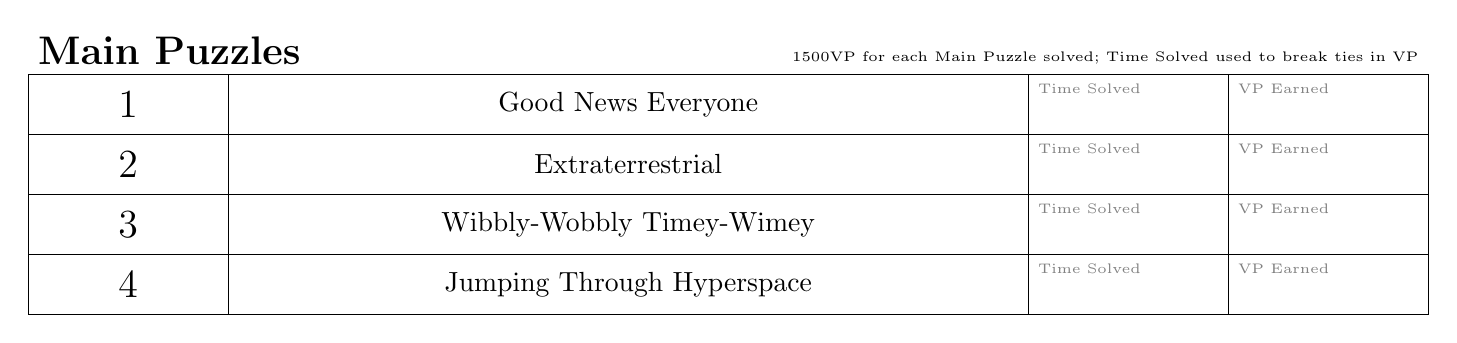
\begin{tikzpicture}[x=1in,y=-0.3in]
  \node[anchor=south west] at (0,0) {\Large\textbf{Main Puzzles}};
  \draw (0,0) rectangle +(7,1);
  \draw (0,1) rectangle +(7,1);
  \draw (0,2) rectangle +(7,1);
  \draw (0,3) rectangle +(7,1);
  \draw (1,0) -- +(0,4);
  \draw (5,0) -- +(0,4);
  \draw (6,0) -- +(0,4);
  \node at (0.5,0.5) {\Large 1};
  \node at (0.5,1.5) {\Large 2};
  \node at (0.5,2.5) {\Large 3};
  \node at (0.5,3.5) {\Large 4};
  \node at (3,0.5) {Good News Everyone};
  \node at (3,1.5) {Extraterrestrial};
  \node at (3,2.5) {Wibbly-Wobbly Timey-Wimey};
  \node at (3,3.5) {Jumping Through Hyperspace};
  \node[color=gray,anchor=north west] at (5,0)
    {\tiny Time Solved};
  \node[color=gray,anchor=north west] at (5,1)
    {\tiny Time Solved};
  \node[color=gray,anchor=north west] at (5,2)
    {\tiny Time Solved};
  \node[color=gray,anchor=north west] at (5,3)
    {\tiny Time Solved};
  \node[color=gray,anchor=north west] at (6,0)
    {\tiny VP Earned};
  \node[color=gray,anchor=north west] at (6,1)
    {\tiny VP Earned};
  \node[color=gray,anchor=north west] at (6,2)
    {\tiny VP Earned};
  \node[color=gray,anchor=north west] at (6,3)
    {\tiny VP Earned};
  \node[anchor=south east] at (7,0)
    {\tiny 1500VP for each Main Puzzle solved;
    Time Solved used to break ties in VP};
\end{tikzpicture}

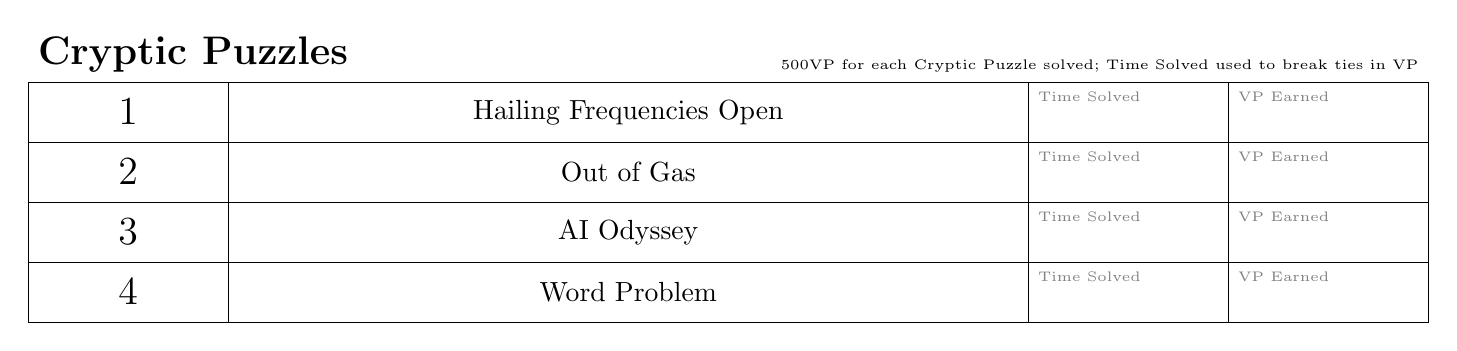
\begin{tikzpicture}[x=1in,y=-0.3in]
  \node[anchor=south west] at (0,0) {\Large\textbf{Cryptic Puzzles}};
  \draw (0,0) rectangle +(7,1);
  \draw (0,1) rectangle +(7,1);
  \draw (0,2) rectangle +(7,1);
  \draw (0,3) rectangle +(7,1);
  \draw (1,0) -- +(0,4);
  \draw (5,0) -- +(0,4);
  \draw (6,0) -- +(0,4);
  \node at (0.5,0.5) {\Large 1};
  \node at (0.5,1.5) {\Large 2};
  \node at (0.5,2.5) {\Large 3};
  \node at (0.5,3.5) {\Large 4};
  \node at (3,0.5) {Hailing Frequencies Open};
  \node at (3,1.5) {Out of Gas};
  \node at (3,2.5) {AI Odyssey};
  \node at (3,3.5) {Word Problem};
  \node[color=gray,anchor=north west] at (5,0)
    {\tiny Time Solved};
  \node[color=gray,anchor=north west] at (5,1)
    {\tiny Time Solved};
  \node[color=gray,anchor=north west] at (5,2)
    {\tiny Time Solved};
  \node[color=gray,anchor=north west] at (5,3)
    {\tiny Time Solved};
  \node[color=gray,anchor=north west] at (6,0)
    {\tiny VP Earned};
  \node[color=gray,anchor=north west] at (6,1)
    {\tiny VP Earned};
  \node[color=gray,anchor=north west] at (6,2)
    {\tiny VP Earned};
  \node[color=gray,anchor=north west] at (6,3)
    {\tiny VP Earned};
  \node[anchor=south east] at (7,0)
    {\tiny 500VP for each Cryptic Puzzle solved;
    Time Solved used to break ties in VP};
\end{tikzpicture}

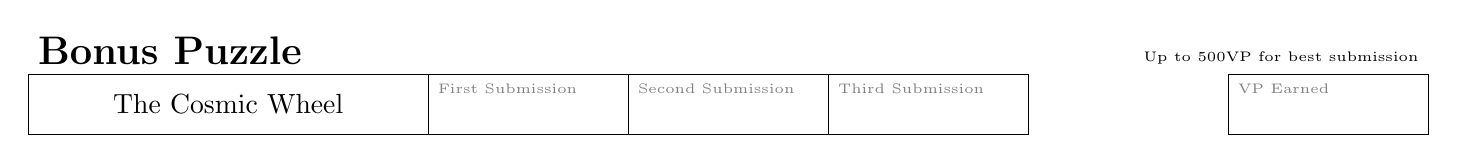
\begin{tikzpicture}[x=1in,y=-0.3in]
  \node[anchor=south west] at (0,0) {\Large\textbf{Bonus Puzzle}};
  \draw (0,0) rectangle +(5,1);
  \draw (2,0) -- +(0,1);
  \draw (3,0) -- +(0,1);
  \draw (4,0) -- +(0,1);
  \draw (6,0) rectangle +(1,1);
  \node at (1,0.5) {The Cosmic Wheel};
  \node[color=gray,anchor=north west] at (2,0)
    {\tiny First Submission};
  \node[color=gray,anchor=north west] at (3,0)
    {\tiny Second Submission};
  \node[color=gray,anchor=north west] at (4,0)
    {\tiny Third Submission};
  \node[color=gray,anchor=north west] at (6,0)
    {\tiny VP Earned};
  \node[anchor=south east] at (7,0)
    {\tiny Up to 500VP for best submission};
\end{tikzpicture}

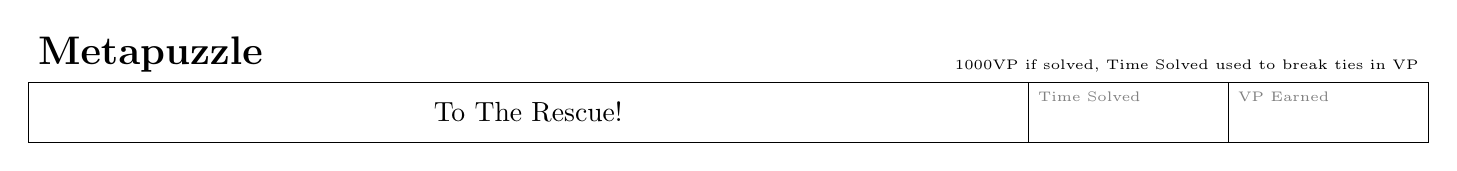
\begin{tikzpicture}[x=1in,y=-0.3in]
  \node[anchor=south west] at (0,0) {\Large\textbf{Metapuzzle}};
  \draw (0,0) rectangle +(7,1);
  \draw (5,0) -- +(0,1);
  \draw (6,0) -- +(0,1);
  \node at (2.5,0.5) {To The Rescue!};
  \node[color=gray,anchor=north west] at (5,0)
    {\tiny Time Solved};
  \node[color=gray,anchor=north west] at (6,0)
    {\tiny VP Earned};
  \node[anchor=south east] at (7,0)
    {\tiny 1000VP if solved,
    Time Solved used to break ties in VP};
\end{tikzpicture}

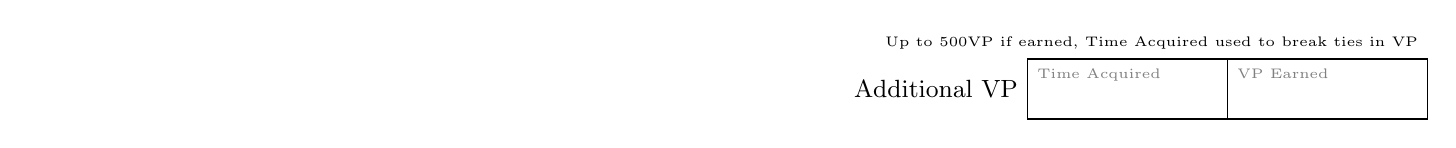
\begin{tikzpicture}[x=1in,y=-0.3in]
  \fill[color=white] (0,0) rectangle +(7,1);
  \draw (5,0) rectangle +(2,1);
  \draw (6,0) -- +(0,1);
  \node[color=gray,anchor=north west] at (5,0)
    {\tiny Time Acquired};
  \node[color=gray,anchor=north west] at (6,0)
    {\tiny VP Earned};
  \node[anchor=south east] at (7,0)
    {\tiny Up to 500VP if earned,
    Time Acquired used to break ties in VP};
  \node[anchor=east] at (5,0.5) {\small Additional VP};
\end{tikzpicture}

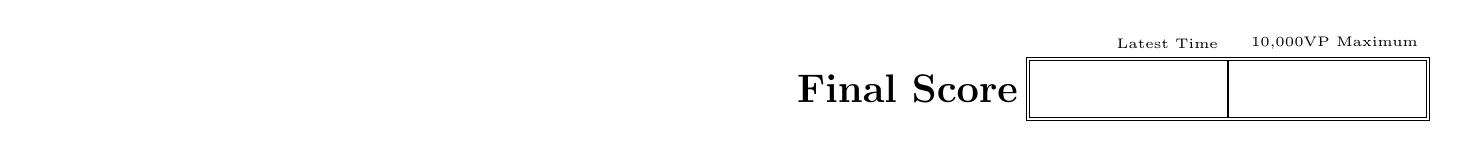
\begin{tikzpicture}[x=1in,y=-0.3in]
  \fill[color=white] (0,0) rectangle +(7,1);
  \draw[thick] (6,0) -- (6,1);
  \draw[double] (5,0) rectangle +(2,1);
  \node[anchor=east] at (5,0.5) {\Large\textbf{Final Score}};
  \node[anchor=south east] at (6,0)
    {\tiny Latest Time};
  \node[anchor=south east] at (7,0)
    {\tiny 10,000VP Maximum};
\end{tikzpicture}

%
% \vspace{1em}
%
% {\noindent\LARGE Team Number: \underline{\hspace{0.5in}}
% School Name: \underline{\hspace{3in}}}


%%% Local Variables:
%%% mode: latex
%%% TeX-master: "../mapp-hsc17-game-book"
%%% End:


\phPart{Puzzles}

\phChapterWorksheet{Where No One Has Gone Before}{Opening Puzzle}

  Today's adventure begins as your team's ship launches into space.
Space Fleet has provided you a 
\textbf{Galaxy Map} to guide you on your way.
(Actually, several copies have been provided to you! Take care of
these copies, as you will refer to the Galaxy Map several times 
throughout the adventure.) Each dot on the map refers to a
different solar system, named on the map.

Space Fleet commands you to first visit the four 
\textbf{Core Systems} of
the galaxy. You can recognize a Core System by the fact that
it is located in the middle of a regular polygon
(all sides are the same length) formed by
either three, four, five, or seven other systems. An
example is shown below.

\begin{center}
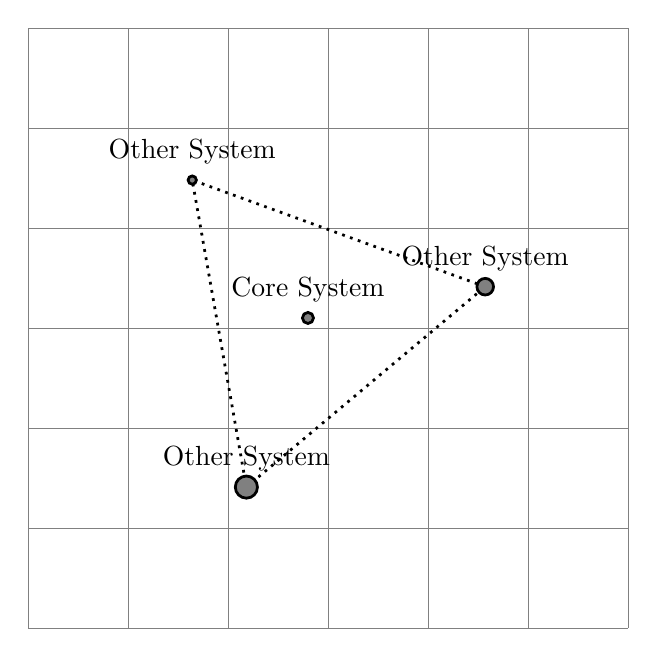
\begin{tikzpicture}[x=0.5in,y=0.5in]
\draw[step=1,gray,very thin] (-3,-3) grid (3,3);
\begin{scope}[
every path/.style={line width=1pt,fill=gray},
shift={(-0.2,0.1)}
]
  %3-gon
  \coordinate (3GonCenter) at (0,0);
  \coordinate (3GonVertex0) at (10:1.8);
  \coordinate (3GonVertex1) at (130:1.8);
  \coordinate (3GonVertex2) at (250:1.8);
  \draw[dotted,fill=none]
    (3GonVertex0) --
    (3GonVertex1) --
    (3GonVertex2) --
    cycle;
  \draw (3GonCenter) node[above=2pt] {Core System} circle (2pt); 
  \draw (3GonVertex0) node[above=2pt] {Other System} circle (3pt); 
  \draw (3GonVertex1) node[above=2pt] {Other System} circle (1.5pt); 
  \draw (3GonVertex2) node[above=2pt] {Other System} circle (4pt);
\end{scope}
\end{tikzpicture}
\end{center}



  \phWorksheet{Galaxy Chart}

  \begin{center}
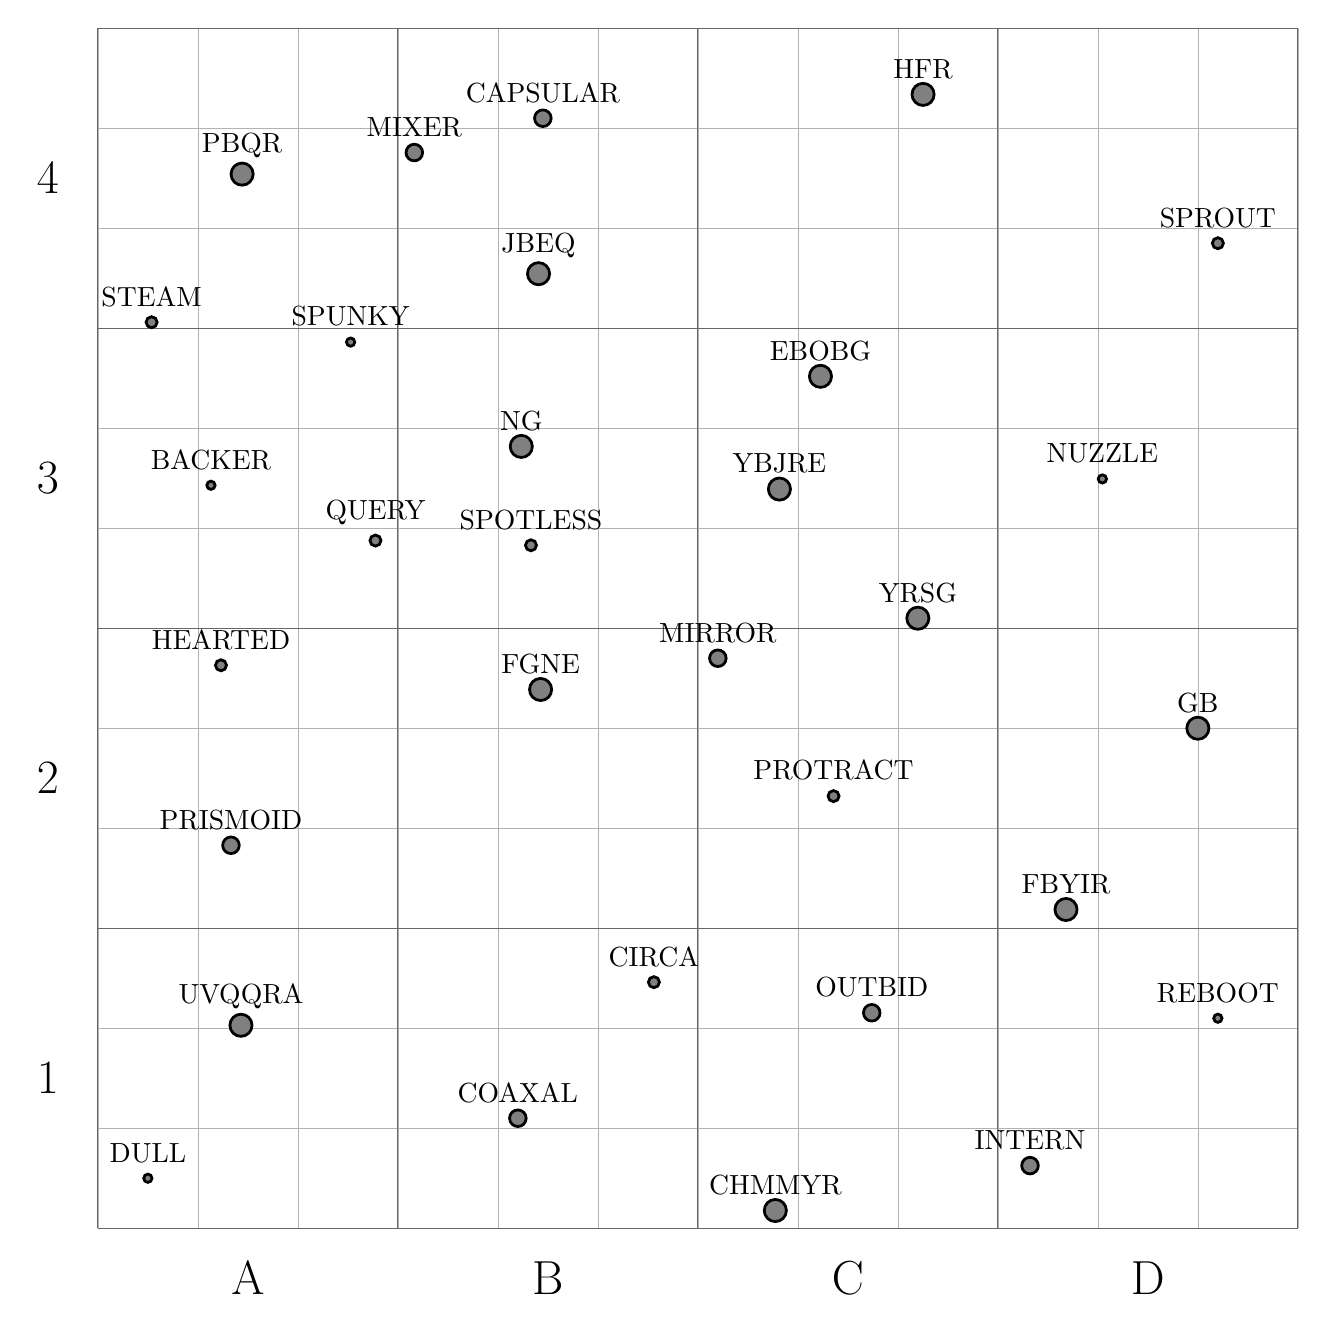
\begin{tikzpicture}[x=0.5in,y=0.5in]
\fill[white] (-6,-6) rectangle (6,6);
\draw[step=1,black!30,very thin] (-6,-6) grid (6,6);
\draw[step=3,black!60,thin] (-6,-6) grid (6,6);
\node at (-4.5,-6.5) {\LARGE A};
\node at (-1.5,-6.5) {\LARGE B};
\node at (1.5,-6.5) {\LARGE C};
\node at (4.5,-6.5) {\LARGE D};
\node at (-6.5,-4.5) {\LARGE 1};
\node at (-6.5,-1.5) {\LARGE 2};
\node at (-6.5,1.5) {\LARGE 3};
\node at (-6.5,4.5) {\LARGE 4};
\coordinate (gridStar) at (5,-1);
\draw[line width=1pt,fill=gray] (gridStar) node[above=2pt] {GB} circle (4pt); 
\coordinate (lowerLeftStar) at (-5.5,-5.5);
\draw[line width=1pt,fill=gray] (lowerLeftStar) node[above=2pt] {DULL} circle (1.5pt); 
\begin{scope}[
every path/.style={line width=1pt,fill=gray},
%every path/.style={line width=1pt,fill=cyan},
shift={(2.2,0.1)}
]
  \coordinate (MetaCenter) at (0,0);
  \coordinate (Meta0) at (3,3.75);
  \coordinate (Meta1) at (-4,-5);
  \coordinate (Meta2) at (-3.75,5);
  \coordinate (Meta3) at (3,-4);
%  \draw[dashdotted,fill=none]
%    (Meta0) --
%    (Meta1);
%  \draw[dashdotted,fill=none]
%    (Meta2) --
%    (Meta3);
  \draw (MetaCenter) node[above=2pt] {YRSG} circle (4pt);%hidden 
  \draw (Meta0) node[above=2pt] {SPROUT} circle (2pt); 
  \draw (Meta1) node[above=2pt] {COAXAL} circle (3pt); 
  \draw (Meta2) node[above=2pt] {CAPSULAR} circle (3pt); 
  \draw (Meta3) node[above=2pt] {REBOOT} circle (1.5pt); 
\end{scope}
\begin{scope}[
every path/.style={line width=1pt,fill=gray},
%every path/.style={line width=1pt,fill=blue},
shift={(0.2,-0.3)}
]
  %3-gon
  \coordinate (3GonCenter) at (0,0);
  \coordinate (3GonVertex0) at (-50:1.8);
  \coordinate (3GonVertex1) at (70:1.8);
  \coordinate (3GonVertex2) at (190:1.8);
%  \draw[dotted,fill=none]
%    (3GonVertex0) --
%    (3GonVertex1) --
%    (3GonVertex2) --
%    cycle;
  \draw (3GonCenter) node[above=2pt] {MIRROR} circle (3pt); 
  \draw (3GonVertex0) node[above=2pt] {PROTRACT} circle (2pt); 
  \draw (3GonVertex1) node[above=2pt] {YBJRE} circle (4pt); %hidden
  \draw (3GonVertex2) node[above=2pt] {FGNE} circle (4pt);%hidden
  
  %4-gon
  \begin{scope}[
  every path/.style={line width=1pt,fill=gray},
%  every path/.style={line width=1pt,fill=green},
  shift={(70:3)}
  ]
    \coordinate (4GonCenter) at (0,0);
    \coordinate (4GonVertex0) at (3GonCenter);
    \coordinate (4GonVertex1) at (-20:3);
    \coordinate (4GonVertex2) at (70:3);
    \coordinate (4GonVertex3) at (160:3);
%    \draw[dotted,fill=none]
%      (4GonVertex0) --
%      (4GonVertex1) --
%      (4GonVertex2) --
%      (4GonVertex3) --
%      cycle;
    \draw (4GonCenter) node[above=2pt] {EBOBG} circle (4pt);  %hidden
    \draw (4GonVertex1) node[above=2pt] {NUZZLE} circle (1.5pt); 
    \draw (4GonVertex2) node[above=2pt] {HFR} circle (4pt);  %hidden
    \draw (4GonVertex3) node[above=2pt] {JBEQ} circle (4pt);  %hidden

    %7-gon
    \begin{scope}[shift={(4GonVertex3)}]\begin{scope}[
    every path/.style={line width=1pt,fill=gray},
%    every path/.style={line width=1pt,fill=yellow},
    shift={(-160:2)}
    ]
      \coordinate (7GonCenter) at (0,0);
      \coordinate (7GonVertex0) at (4GonVertex3);
      \coordinate (7GonVertex1) at (71.43:2);
      \coordinate (7GonVertex2) at (122.86:2);
      \coordinate (7GonVertex3) at (174.29:2);
      \coordinate (7GonVertex4) at (225.71:2);
      \coordinate (7GonVertex5) at (277.14:2);
      \coordinate (7GonVertex6) at (328.57:2);
%      \draw[dotted,fill=none]
%        (7GonVertex0) --
%        (7GonVertex1) --
%        (7GonVertex2) --
%        (7GonVertex3) --
%        (7GonVertex4) --
%        (7GonVertex5) --
%        (7GonVertex6) --
%        cycle;
      \draw (7GonCenter) node[above=2pt] {SPUNKY} circle (1.5pt); 
      \draw (7GonVertex1) node[above=2pt] {MIXER} circle (3pt); 
      \draw (7GonVertex2) node[above=2pt] {PBQR} circle (4pt);  %hidden
      \draw (7GonVertex3) node[above=2pt] {STEAM} circle (2pt); 
      \draw (7GonVertex4) node[above=2pt] {BACKER} circle (1.5pt); 
      \draw (7GonVertex5) node[above=2pt] {QUERY} circle (2pt); 
      \draw (7GonVertex6) node[above=2pt] {NG} circle (4pt);%hidden

      %line
      \begin{scope}[
      every path/.style={line width=1pt,fill=gray},
%      every path/.style={line width=1pt,fill=purple},
      shift={(7GonVertex4)}
      ]
        \coordinate (lineStar0) at (0,0);
        \coordinate (lineStar1) at (0.1,-1.8);
        \coordinate (lineStar2) at (0.2,-3.6);
        \coordinate (lineStar3) at (0.3,-5.4);
%        \draw[dashed,fill=none]
%          (lineStar0) --
%          (lineStar1) --
%          (lineStar2) --
%          (lineStar3);
        \draw (lineStar1) node[above=2pt] {HEARTED} circle (2pt); 
        \draw (lineStar2) node[above=2pt] {PRISMOID} circle (3pt); 
        \draw (lineStar3) node[above=2pt] {UVQQRA} circle (4pt);%hidden

        %vector
%        \draw[dashed] (lineStar2) -- +(3,3);
        \node (vectorStar) at ($(lineStar2)+(3,3)$) {}; 
        \draw[line width=1pt,fill=gray] (vectorStar) node[above=2pt] {SPOTLESS} circle (2pt);
      \end{scope}
    \end{scope}\end{scope}
  \end{scope}

  %5-gon
  \begin{scope}[shift={(3GonVertex0)}]\begin{scope}[
  every path/.style={line width=1pt,fill=gray},
%  every path/.style={line width=1pt,fill=red},
  shift={(-80:2.2)}
  ]
    \coordinate (5GonCenter) at (0,0);
    \coordinate (5GonVertex0) at (28:2.2);
    \coordinate (5GonVertex1) at (3GonVertex0);
    \coordinate (5GonVertex2) at (172:2.2);
    \coordinate (5GonVertex3) at (244:2.2);
    \coordinate (5GonVertex4) at (316:2.2);
%    \draw[dotted,fill=none]
%      (5GonVertex0) --
%      (5GonVertex1) --
%      (5GonVertex2) --
%      (5GonVertex3) --
%      (5GonVertex4) --
%      cycle;
    \draw (5GonCenter) node[above=2pt] {OUTBID} circle (3pt);
    \draw (5GonVertex0) node[above=2pt] {FBYIR} circle (4pt);%hidden
    \draw (5GonVertex2) node[above=2pt] {CIRCA} circle (2pt);
    \draw (5GonVertex3) node[above=2pt] {CHMMYR} circle (4pt);%hidden
    \draw (5GonVertex4) node[above=2pt] {INTERN} circle (3pt);
  \end{scope}\end{scope}
%    \foreach \a in {28,100,172,244,316} { %\a is the angle variable
%      \draw[line width=1pt,fill=red] (\a:2.2) circle (3pt);
%    }
\end{scope}
\end{tikzpicture}
\end{center}


% USE CODE WORD ROBOT AT LOWER LEFT STAR TO SOLVE HIDDEN PUZZLE
% HFR PBQR JBEQ EBOBG NG YBJRE YRSG FGNE GB FBYIR UVQQRA CHMMYR


\phChapterWorksheet{Good News Everyone}{Main Puzzle 1}

  On this system, you find yourself caught up in the misadventures of
PlanEx, an
intergalactic delivery company led by the eccentric old mathematician
Dr. Farnswell. In the name of good relations between galaxies, you
agree to help him with the following puzzle. 

\begin{itemize}
\item PlanEx makes deliveries
to six different planets (not including their own) on Mondays, Wednesdays,
and Fridays. 
\item Each day, a different company on each planet receives the
delivery, listed below in order of Mon/Wed/Fri.
\begin{itemize}
\item Planet 1: Venus Co. / Rave Co. / Photon Co.
\item Planet 2: Comet Co. / Solar Co. / Light Co.
\item Planet 3: Belt Co. / Techno Co. / Alarm Co.
\item Planet 4: Acme Co. / Alpha Co. / Uranium Co.
\item Planet 5: Oxygen Co. / Helmet Co. / Neo Co.
\item Planet 6: Star Co. / Orion Co. / Tele Co.
\end{itemize}
\item Their ship may travel directly between any two planets,
  but due to galactic regulations, they may not travel directly
  between the same two planets twice in the same week, regardless
  of direction. This restriction includes travel to/from the Home Planet.
\end{itemize}

Can you help Farnswell complete his \textbf{Delivery Schedule}? If so,
the missing company names will reveal a hidden codeword. 

\begin{center}
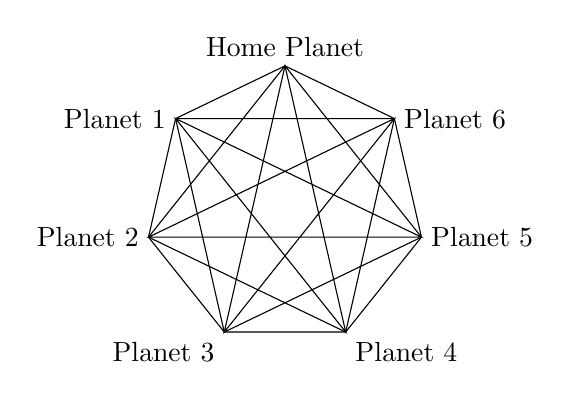
\begin{tikzpicture}[x=0.7in,y=0.7in]
\coordinate (Vertex0) at (90:1);
\coordinate (Vertex1) at (141.4:1);
\coordinate (Vertex2) at (192.9:1);
\coordinate (Vertex3) at (244.3:1);
\coordinate (Vertex4) at (295.7:1);
\coordinate (Vertex5) at (347.1:1);
\coordinate (Vertex6) at (38.6:1);
\node[above] at (Vertex0) {Home Planet};
\node[left] at (Vertex1) {Planet 1};
\node[left] at (Vertex2) {Planet 2};
\node[below left] at (Vertex3) {Planet 3};
\node[below right] at (Vertex4) {Planet 4};
\node[right] at (Vertex5) {Planet 5};
\node[right] at (Vertex6) {Planet 6};
\draw 
  (Vertex0) -- 
  (Vertex1) -- 
  (Vertex2) --
  (Vertex3) -- 
  (Vertex4) -- 
  (Vertex5) --
  (Vertex6) --
  cycle; 
\draw 
  (Vertex0) -- 
  (Vertex2) -- 
  (Vertex4) --
  (Vertex6) -- 
  (Vertex1) -- 
  (Vertex3) --
  (Vertex5) --
  cycle; 
\draw 
  (Vertex0) -- 
  (Vertex3) -- 
  (Vertex6) --
  (Vertex2) -- 
  (Vertex5) -- 
  (Vertex1) --
  (Vertex4) --
  cycle; 
\end{tikzpicture}
\end{center} 


  \phWorksheet{Delivery Schedule}

  \begin{center}
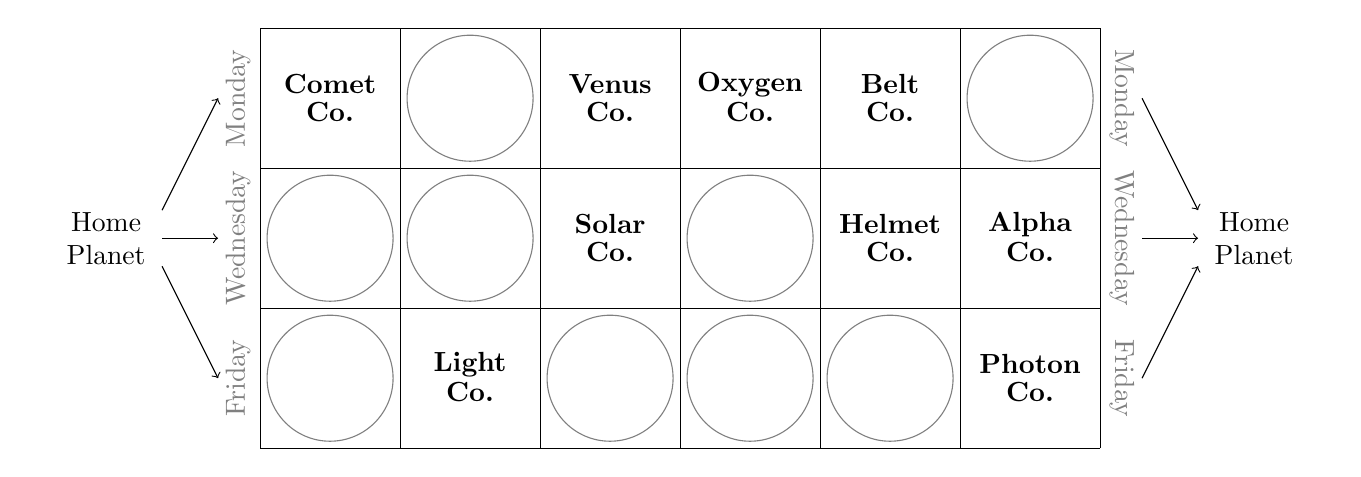
\begin{tikzpicture}[x=0.7in,y=0.7in]
\fill[white] (-4,0) rectangle (4,3);
\draw[step=1,thin] (-3,0) grid (3,3);

\node[text width=5em,align=center] at (-4.1,1.5) {Home\\Planet};
\node[text width=5em,align=center] at (4.1,1.5) {Home\\Planet};
\draw[->] (-3.7,1.7) -- (-3.3,2.5);
\draw[->] (-3.7,1.5) -- (-3.3,1.5);
\draw[->] (-3.7,1.3) -- (-3.3,0.5);
\draw[<-] (3.7,1.7) -- (3.3,2.5);
\draw[<-] (3.7,1.5) -- (3.3,1.5);
\draw[<-] (3.7,1.3) -- (3.3,0.5);

\node[color=gray,anchor=east] at (-3,2.5) {\rotatebox{90}{Monday}};
\node[color=gray,anchor=east] at (-3,1.5) {\rotatebox{90}{Wednesday}};
\node[color=gray,anchor=east] at (-3,0.5) {\rotatebox{90}{Friday}};
\node[color=gray,anchor=west] at (3,2.5) {\rotatebox{270}{Monday}};
\node[color=gray,anchor=west] at (3,1.5) {\rotatebox{270}{Wednesday}};
\node[color=gray,anchor=west] at (3,0.5) {\rotatebox{270}{Friday}};

%\node[color=gray,anchor=south] at (-2.5,3) {1st};
%\node[color=gray,anchor=south] at (-1.5,3) {2nd};
%\node[color=gray,anchor=south] at (-0.5,3) {3rd};
%\node[color=gray,anchor=south] at (0.5,3) {4th};
%\node[color=gray,anchor=south] at (1.5,3) {5th};
%\node[color=gray,anchor=south] at (2.5,3) {6th};

\draw[color=gray] (-1.5,2.5) circle (0.45);
\draw[color=gray] (2.5,2.5) circle (0.45);
\draw[color=gray] (-2.5,1.5) circle (0.45);
\draw[color=gray] (-1.5,1.5) circle (0.45);
\draw[color=gray] (0.5,1.5) circle (0.45);
\draw[color=gray] (-2.5,0.5) circle (0.45);
\draw[color=gray] (-0.5,0.5) circle (0.45);
\draw[color=gray] (0.5,0.5) circle (0.45);
\draw[color=gray] (1.5,0.5) circle (0.45);

\node at (-2.5,2.6) {\textbf{Comet}};
\node at (-2.5,2.4) {\textbf{Co.}};
\node at (-0.5,2.6) {\textbf{Venus}};
\node at (-0.5,2.4) {\textbf{Co.}};
\node at (0.5,2.6) {\textbf{Oxygen}};
\node at (0.5,2.4) {\textbf{Co.}};
\node at (1.5,2.6) {\textbf{Belt}};
\node at (1.5,2.4) {\textbf{Co.}};

\node at (-0.5,1.6) {\textbf{Solar}};
\node at (-0.5,1.4) {\textbf{Co.}};
\node at (1.5,1.6) {\textbf{Helmet}};
\node at (1.5,1.4) {\textbf{Co.}};
\node at (2.5,1.6) {\textbf{Alpha}};
\node at (2.5,1.4) {\textbf{Co.}};

\node at (-1.5,0.6) {\textbf{Light}};
\node at (-1.5,0.4) {\textbf{Co.}};
\node at (2.5,0.6) {\textbf{Photon}};
\node at (2.5,0.4) {\textbf{Co.}};

%SOLUTION
%\node at (-1.5,2.5) {\textbf{Acme}};
%\node at (2.5,2.5) {\textbf{Star}};
%\node at (-2.5,1.5) {\textbf{Techno}};
%\node at (-1.5,1.5) {\textbf{Rave}};
%\node at (0.5,1.5) {\textbf{Orion}};
%\node at (-2.5,0.5) {\textbf{Neo}};
%\node at (-0.5,0.5) {\textbf{Alarm}};
%\node at (0.5,0.5) {\textbf{Uranium}};
%\node at (1.5,0.5) {\textbf{Tele}};
%\node[above] at (-2.5,2) {2};
%\node[above] at (-1.5,2) {4};
%\node[above] at (-0.5,2) {1};
%\node[above] at (0.5,2)  {5};
%\node[above] at (1.5,2)  {3};
%\node[above] at (2.5,2)  {6};
%\node[above] at (-2.5,1) {3};
%\node[above] at (-1.5,1) {1};
%\node[above] at (-0.5,1) {2};
%\node[above] at (0.5,1)  {6};
%\node[above] at (1.5,1)  {5};
%\node[above] at (2.5,1)  {4};
%\node[above] at (-2.5,0) {5};
%\node[above] at (-1.5,0) {2};
%\node[above] at (-0.5,0) {3};
%\node[above] at (0.5,0)  {4};
%\node[above] at (1.5,0)  {6};
%\node[above] at (2.5,0)  {1};
\end{tikzpicture}
\end{center}


  \phWorksheet{Solution}

  The numbers below coorrespond to each company's planet.

\begin{center}
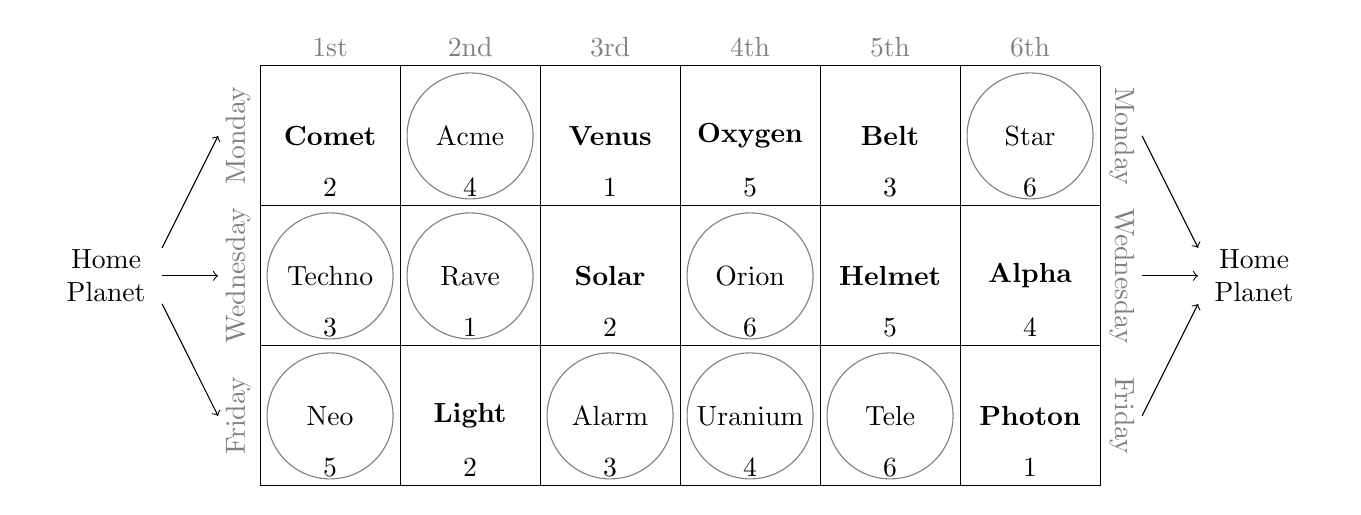
\begin{tikzpicture}[x=0.7in,y=0.7in]
\fill[white] (-4,0) rectangle (4,3);
\draw[step=1,thin] (-3,0) grid (3,3);

\node[text width=5em,align=center] at (-4.1,1.5) {Home\\Planet};
\node[text width=5em,align=center] at (4.1,1.5) {Home\\Planet};
\draw[->] (-3.7,1.7) -- (-3.3,2.5);
\draw[->] (-3.7,1.5) -- (-3.3,1.5);
\draw[->] (-3.7,1.3) -- (-3.3,0.5);
\draw[<-] (3.7,1.7) -- (3.3,2.5);
\draw[<-] (3.7,1.5) -- (3.3,1.5);
\draw[<-] (3.7,1.3) -- (3.3,0.5);

\node[color=gray,anchor=east] at (-3,2.5) {\rotatebox{90}{Monday}};
\node[color=gray,anchor=east] at (-3,1.5) {\rotatebox{90}{Wednesday}};
\node[color=gray,anchor=east] at (-3,0.5) {\rotatebox{90}{Friday}};
\node[color=gray,anchor=west] at (3,2.5) {\rotatebox{270}{Monday}};
\node[color=gray,anchor=west] at (3,1.5) {\rotatebox{270}{Wednesday}};
\node[color=gray,anchor=west] at (3,0.5) {\rotatebox{270}{Friday}};

\node[color=gray,anchor=south] at (-2.5,3) {1st};
\node[color=gray,anchor=south] at (-1.5,3) {2nd};
\node[color=gray,anchor=south] at (-0.5,3) {3rd};
\node[color=gray,anchor=south] at (0.5,3) {4th};
\node[color=gray,anchor=south] at (1.5,3) {5th};
\node[color=gray,anchor=south] at (2.5,3) {6th};

\draw[color=gray] (-1.5,2.5) circle (0.45);
\draw[color=gray] (2.5,2.5) circle (0.45);
\draw[color=gray] (-2.5,1.5) circle (0.45);
\draw[color=gray] (-1.5,1.5) circle (0.45);
\draw[color=gray] (0.5,1.5) circle (0.45);
\draw[color=gray] (-2.5,0.5) circle (0.45);
\draw[color=gray] (-0.5,0.5) circle (0.45);
\draw[color=gray] (0.5,0.5) circle (0.45);
\draw[color=gray] (1.5,0.5) circle (0.45);

\node at (-2.5,2.5) {\textbf{Comet}};
\node at (-0.5,2.5) {\textbf{Venus}};
\node at (0.5,2.5) {\textbf{Oxygen}};
\node at (1.5,2.5) {\textbf{Belt}};

\node at (-0.5,1.5) {\textbf{Solar}};
\node at (1.5,1.5) {\textbf{Helmet}};
\node at (2.5,1.5) {\textbf{Alpha}};

\node at (-1.5,0.5) {\textbf{Light}};
\node at (2.5,0.5) {\textbf{Photon}};

%SOLUTION
\node at (-1.5,2.5) {Acme};
\node at (2.5,2.5) {Star};
\node at (-2.5,1.5) {Techno};
\node at (-1.5,1.5) {Rave};
\node at (0.5,1.5) {Orion};
\node at (-2.5,0.5) {Neo};
\node at (-0.5,0.5) {Alarm};
\node at (0.5,0.5) {Uranium};
\node at (1.5,0.5) {Tele};
\node[above] at (-2.5,2) {2};
\node[above] at (-1.5,2) {4};
\node[above] at (-0.5,2) {1};
\node[above] at (0.5,2)  {5};
\node[above] at (1.5,2)  {3};
\node[above] at (2.5,2)  {6};
\node[above] at (-2.5,1) {3};
\node[above] at (-1.5,1) {1};
\node[above] at (-0.5,1) {2};
\node[above] at (0.5,1)  {6};
\node[above] at (1.5,1)  {5};
\node[above] at (2.5,1)  {4};
\node[above] at (-2.5,0) {5};
\node[above] at (-1.5,0) {2};
\node[above] at (-0.5,0) {3};
\node[above] at (0.5,0)  {4};
\node[above] at (1.5,0)  {6};
\node[above] at (2.5,0)  {1};
\end{tikzpicture}
\end{center}

Using the first letters of the filled-in company names, the solution
\texttt{ASTRONAUT} is revealed.


\phChapterWorksheet{No One Can Hear You Scream}{Main Puzzle 2}

  The one golden rule of space travel is simple: if you find a creepy
egg on a previously unexplored planet, DO NOT TAKE IT BACK WITH YOU.
Well, it seems Ensign S. Ridley didn't get the memo, as after
a routine check on one of this system's planets, your crew finds
themselves running for their lives as a mysterious alien
rampages your ship!

Fortunately, there is protocol for such a situation. On your
\textbf{Ship Floorplan}, several stations are marked where you
can position a robotic guard to defend against the alien. 
Five guards must be placed such that every point within the floorplan
is visible in a straight line from at least one guard.

An example for two guards is illustrated below. As long as one
guard is placed within the top two rows, and the other guard is
placed within the bottom two rows, the entire area of the floor
is safely monitored. But if a guard is placed on any of the
three stations in the middle row,
there's no possible way for a second guard to monitor both
the top and bottom unaccounted areas.

Your task is to identify all the stations on the ship that
are unusable. In addition to saving your crew from
certain death, you will also reveal a secret codeword!

\newcommand{\hysExample}{
\draw[line width=2pt]
  (0,3) --
  (3,6) --
  (7,6) --
  (7,3.5) --
  (4,3.5) --
  (4,2.5) --
  (7,2.5) --
  (7,0) --
  (3,0) --
  cycle;
\draw[fill=black!20] (3,1) circle (0.1);
\draw[fill=black!20] (4,1) circle (0.1);
\draw[fill=black!20] (5,1) circle (0.1);
\draw[fill=black!20] (6,1) circle (0.1);
\draw[fill=black!20] (2,2) circle (0.1);
\draw[fill=black!20] (3,2) circle (0.1);
\draw[fill=black!20] (1,3) circle (0.1);
\draw[fill=black!20] (2,3) circle (0.1);
\draw[fill=black!20] (3,3) circle (0.1);
\draw[fill=black!20] (2,4) circle (0.1);
\draw[fill=black!20] (3,4) circle (0.1);
\draw[fill=black!20] (3,5) circle (0.1);
\draw[fill=black!20] (4,5) circle (0.1);
\draw[fill=black!20] (5,5) circle (0.1);
\draw[fill=black!20] (6,5) circle (0.1);
}
\begin{center}
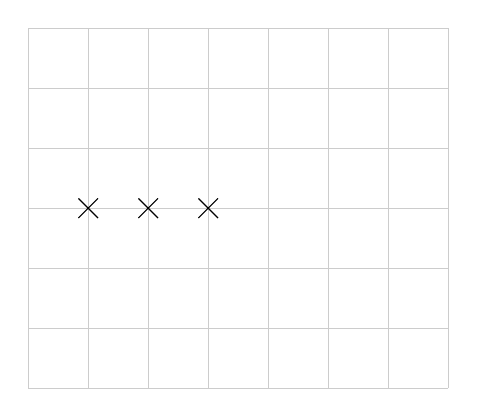
\begin{tikzpicture}[x=0.3in,y=0.3in]
\fill[white] (0,0) rectangle (7,6);
\draw[step=1,thin,black!20] (0,0) grid (7,6);
\hysExample
%\node[anchor=north] at (4,0) {2 guards, 3 unusable stations};
\node[draw,cross out] at (1,3) {};
\node[draw,cross out] at (2,3) {};
\node[draw,cross out] at (3,3) {};
\end{tikzpicture}

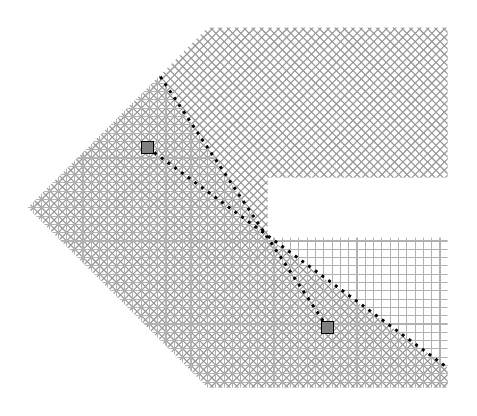
\begin{tikzpicture}[x=0.3in,y=0.3in]
\fill[white] (0,0) rectangle (7,6);
\fill[pattern=crosshatch, pattern color=black!40]
  (7,0.33) --
  (7,0) --
  (3,0) --
  (0,3) --
  (3,6) --
  (7,6) --
  (7,3.5) --
  (4,3.5) --
  (4,2.5) --
  cycle;
\fill[pattern=grid, pattern color=black!30]
  (2.2,5.2) --
  (4,2.5) --
  (7,2.5) --
  (7,0) --
  (3,0) --
  (0,3) --
  cycle;
\draw[line width=1pt,dotted] (2,4) -- (7,0.33);
\draw[line width=1pt,dotted] (5,1) -- (2.2,5.2);
\hysExample
\draw[fill=black!50] (1.9,3.9) rectangle (2.1,4.1);
\draw[fill=black!50] (4.9,0.9) rectangle (5.1,1.1);
\end{tikzpicture}
\hspace{0.2in}
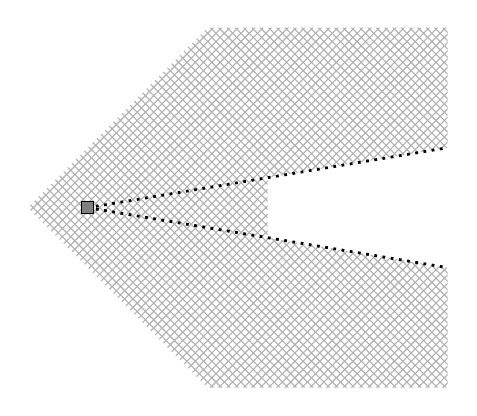
\begin{tikzpicture}[x=0.3in,y=0.3in]
\fill[white] (0,0) rectangle (7,6);
\fill[pattern=crosshatch, pattern color=black!30]
  (0,3) --
  (3,6) --
  (7,6) --
  (7,4) --
  (4,3.5) --
  (4,2.5) --
  (7,2) --
  (7,0) --
  (3,0) --
  cycle;
\draw[line width=1pt,dotted] (1,3) -- (7,4);
\draw[line width=1pt,dotted] (1,3) -- (7,2);
\hysExample
\draw[fill=black!50] (0.9,2.9) rectangle (1.1,3.1);
\end{tikzpicture}
\end{center} 


  \phWorksheet{Ship Floorplan}

  \begin{center}
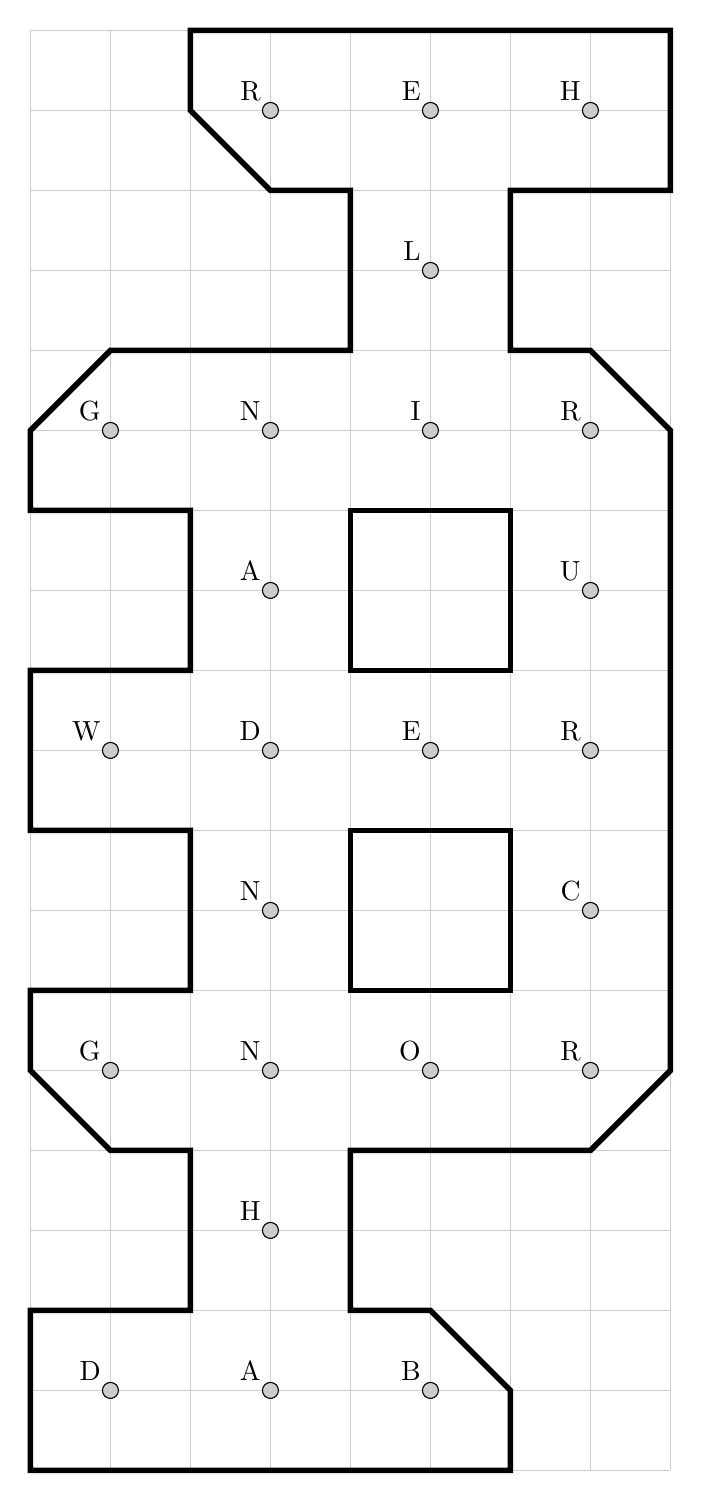
\begin{tikzpicture}[x=0.4in,y=0.4in]
\fill[white] (0,0) rectangle (8,18);
\draw[step=1,thin,black!20] (0,0) grid (8,18);
\draw[line width=2pt]
  (0,0) --
  (6,0) --
  (6,1) --
  (5,2) --
  (4,2) --
  (4,4) --
  (7,4) --
  (8,5) --
  (8,13) --
  (7,14) --
  (6,14) --
  (6,16) --
  (8,16) --
  (8,18) --
  (2,18) --
  (2,17) --
  (3,16) --
  (4,16) --
  (4,14) --
  (1,14) --
  (0,13) --
  (0,12) --
  (2,12) --
  (2,10) --
  (0,10) --
  (0,8) --
  (2,8) --
  (2,6) --
  (0,6) --
  (0,5) --
  (1,4) --
  (2,4) --
  (2,2) --
  (0,2) --
  cycle;
\draw[line width=2pt] (4,6) rectangle (6,8);
\draw[line width=2pt] (4,10) rectangle (6,12);
\draw[fill=black!20] (1,1) node[above left] {D} circle (0.1);
\draw[fill=black!20] (3,1) node[above left] {A} circle (0.1);
\draw[fill=black!20] (5,1) node[above left] {B} circle (0.1);
\draw[fill=black!20] (3,3) node[above left] {H} circle (0.1);
\draw[fill=black!20] (1,5) node[above left] {G} circle (0.1);
\draw[fill=black!20] (3,5) node[above left] {N} circle (0.1);
\draw[fill=black!20] (5,5) node[above left] {O} circle (0.1);
\draw[fill=black!20] (7,5) node[above left] {R} circle (0.1);
\draw[fill=black!20] (3,7) node[above left] {N} circle (0.1);
\draw[fill=black!20] (7,7) node[above left] {C} circle (0.1);
\draw[fill=black!20] (1,9) node[above left] {W} circle (0.1);
\draw[fill=black!20] (3,9) node[above left] {D} circle (0.1);
\draw[fill=black!20] (5,9) node[above left] {E} circle (0.1);
\draw[fill=black!20] (7,9) node[above left] {R} circle (0.1);
\draw[fill=black!20] (3,11) node[above left] {A} circle (0.1);
\draw[fill=black!20] (7,11) node[above left] {U} circle (0.1);
\draw[fill=black!20] (1,13) node[above left] {G} circle (0.1);
\draw[fill=black!20] (3,13) node[above left] {N} circle (0.1);
\draw[fill=black!20] (5,13) node[above left] {I} circle (0.1);
\draw[fill=black!20] (7,13) node[above left] {R} circle (0.1);
\draw[fill=black!20] (5,15) node[above left] {L} circle (0.1);
\draw[fill=black!20] (3,17) node[above left] {R} circle (0.1);
\draw[fill=black!20] (5,17) node[above left] {E} circle (0.1);
\draw[fill=black!20] (7,17) node[above left] {H} circle (0.1);
\end{tikzpicture}
\end{center}


  \phWorksheet{Solution}

  There are six unusable locations.

\begin{center}
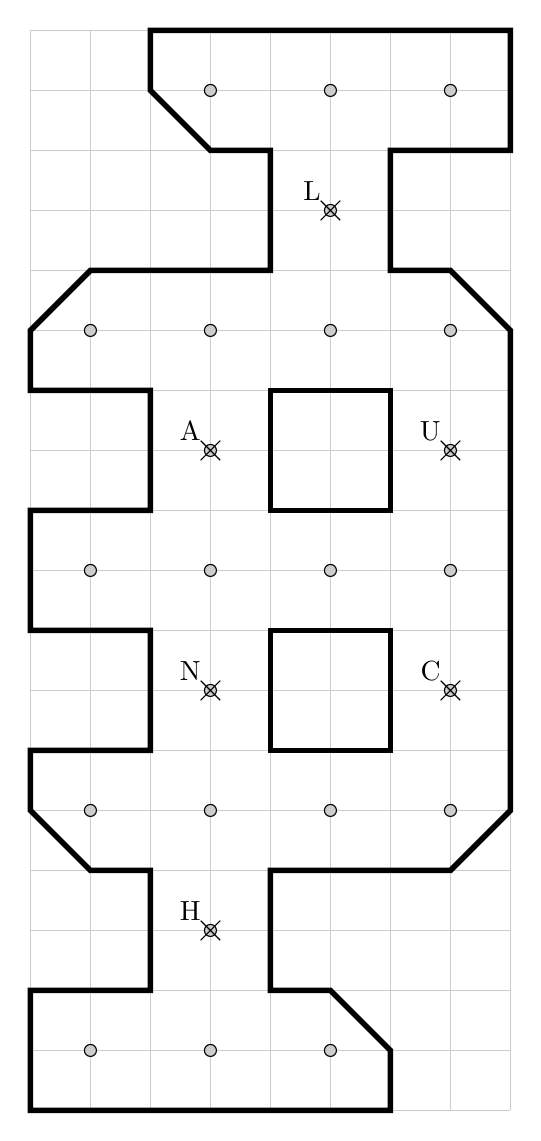
\begin{tikzpicture}[x=0.3in,y=0.3in]
\fill[white] (0,0) rectangle (8,18);
\draw[step=1,thin,black!20] (0,0) grid (8,18);
\draw[line width=2pt]
  (0,0) --
  (6,0) --
  (6,1) --
  (5,2) --
  (4,2) --
  (4,4) --
  (7,4) --
  (8,5) --
  (8,13) --
  (7,14) --
  (6,14) --
  (6,16) --
  (8,16) --
  (8,18) --
  (2,18) --
  (2,17) --
  (3,16) --
  (4,16) --
  (4,14) --
  (1,14) --
  (0,13) --
  (0,12) --
  (2,12) --
  (2,10) --
  (0,10) --
  (0,8) --
  (2,8) --
  (2,6) --
  (0,6) --
  (0,5) --
  (1,4) --
  (2,4) --
  (2,2) --
  (0,2) --
  cycle;
\draw[line width=2pt] (4,6) rectangle (6,8);
\draw[line width=2pt] (4,10) rectangle (6,12);
\draw[fill=black!20] (1,1) node[above left] {} circle (0.1);
\draw[fill=black!20] (3,1) node[above left] {} circle (0.1);
\draw[fill=black!20] (5,1) node[above left] {} circle (0.1);
\draw[fill=black!20] (3,3) node[above left] {H} circle (0.1);
\node[draw,cross out] at (3,3) {};
\draw[fill=black!20] (1,5) node[above left] {} circle (0.1);
\draw[fill=black!20] (3,5) node[above left] {} circle (0.1);
\draw[fill=black!20] (5,5) node[above left] {} circle (0.1);
\draw[fill=black!20] (7,5) node[above left] {} circle (0.1);
\draw[fill=black!20] (3,7) node[above left] {N} circle (0.1);
\node[draw,cross out] at (3,7) {};
\draw[fill=black!20] (7,7) node[above left] {C} circle (0.1);
\node[draw,cross out] at (7,7) {};
\draw[fill=black!20] (1,9) node[above left] {} circle (0.1);
\draw[fill=black!20] (3,9) node[above left] {} circle (0.1);
\draw[fill=black!20] (5,9) node[above left] {} circle (0.1);
\draw[fill=black!20] (7,9) node[above left] {} circle (0.1);
\draw[fill=black!20] (3,11) node[above left] {A} circle (0.1);
\node[draw,cross out] at (3,11) {};
\draw[fill=black!20] (7,11) node[above left] {U} circle (0.1);
\node[draw,cross out] at (7,11) {};
\draw[fill=black!20] (1,13) node[above left] {} circle (0.1);
\draw[fill=black!20] (3,13) node[above left] {} circle (0.1);
\draw[fill=black!20] (5,13) node[above left] {} circle (0.1);
\draw[fill=black!20] (7,13) node[above left] {} circle (0.1);
\draw[fill=black!20] (5,15) node[above left] {L} circle (0.1);
\node[draw,cross out] at (5,15) {};
\draw[fill=black!20] (3,17) node[above left] {} circle (0.1);
\draw[fill=black!20] (5,17) node[above left] {} circle (0.1);
\draw[fill=black!20] (7,17) node[above left] {} circle (0.1);
\end{tikzpicture}
\end{center}

The letters for these stations spell out the solution
\texttt{LAUNCH}.


\phChapterWorksheet{Wibbly-Wobbly Timey-Wimey}{Main Puzzle 3}

  As though it was always destined to happen, your team has encountered
the time-traveling eccentric known only as Professor Whatsit. Well, not
so much ``encountered'' as ``collided'', as witnessed by the 
telephone-booth-shaped breach in your starboard hull.

This whacky master of time with a penchant for fezzes and bow ties promises to
repair your ship, but he first needs your help preventing a
Time Crash. You've never heard of this phenomenon before (he describes it as a
``timey-wimey, wibbly-wobbly sort of thing''), but as it seems to be 
related to a puzzle, you agree to pitch in.

Six parallel dimensions are represented by six groups of numbers on
the \textbf{Dimensional Signals} sheet. In every dimension, this solar system
has six planets; the numbers represent how close their orbit reaches their sun.
As it happens, today all six planets will reach that closest
point, forming a straight line. But because this will happen
in all six dimensions simultaneously, all the planets will begin
to warp and eventually merge into each other!
%
%Your task is to associate each group of numbers with a corresponding
%dimensional signal. This signal is constructed by comparing the relative distances
%between adjacent planets when aligned. The six planets begin mutually
%disconnected, but the Time Crash will cause them to warp and overlap,
%eventually merging all the planets into one! 

Thankfully, you can prevent all of this if you can help the Professor
calculate the dimensional signal that would be caused by this dimensional
warp, spelling out a six-letter hidden codeword!
The signal for each dimension represents how
the planets in a dimension would merge as the warping factor increases,
with merged planets represented by bars and isolated planets represented
by dots (with order not mattering). 
The illustration below demonstrates this effect for \texttt{06-24-32-55-70-99}.

\begin{center}
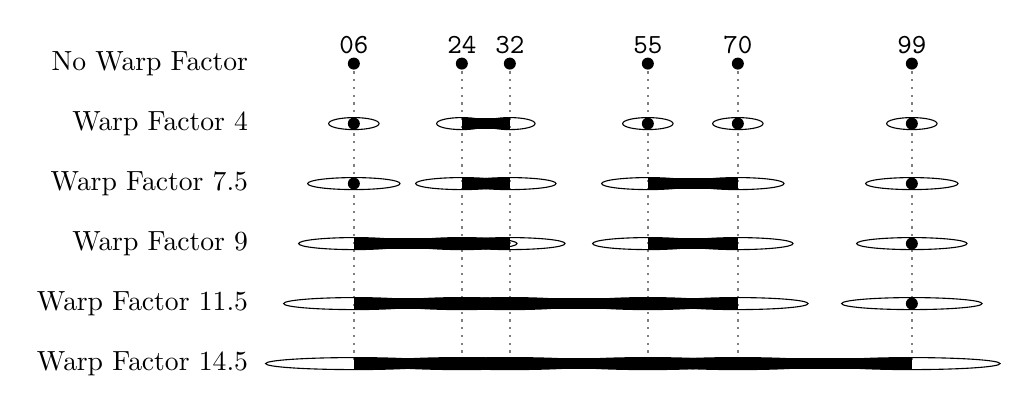
\begin{tikzpicture}[x=0.3in,y=0.3in] 
\node[left] at (-1,0) {No Warp Factor};
\node[left] at (-1,-1) {Warp Factor \(4\)};
\node[left] at (-1,-2) {Warp Factor \(7.5\)};
\node[left] at (-1,-3) {Warp Factor \(9\)};
\node[left] at (-1,-4) {Warp Factor \(11.5\)};
\node[left] at (-1,-5) {Warp Factor \(14.5\)};
\draw[thick,black!50,dotted] (0.6,0) -- +(0,-5);
\draw[thick,black!50,dotted] (2.4,0) -- +(0,-5);
\draw[thick,black!50,dotted] (3.2,0) -- +(0,-5);
\draw[thick,black!50,dotted] (5.5,0) -- +(0,-5);
\draw[thick,black!50,dotted] (7.0,0) -- +(0,-5);
\draw[thick,black!50,dotted] (9.9,0) -- +(0,-5);
\fill (0.6,0) circle (0.1) node[above] {\texttt{06}};
\fill (2.4,0) circle (0.1) node[above] {\texttt{24}};
\fill (3.2,0) circle (0.1) node[above] {\texttt{32}};
\fill (5.5,0) circle (0.1) node[above] {\texttt{55}};
\fill (7.0,0) circle (0.1) node[above] {\texttt{70}};
\fill (9.9,0) circle (0.1) node[above] {\texttt{99}};
\begin{scope}[shift={(0,-1)}]
\draw (0.6,0) ellipse (0.42 and 0.1); 
\draw (2.4,0) ellipse (0.42 and 0.1); 
\draw (3.2,0) ellipse (0.42 and 0.1); 
\draw (5.5,0) ellipse (0.42 and 0.1); 
\draw (7.0,0) ellipse (0.42 and 0.1); 
\draw (9.9,0) ellipse (0.42 and 0.1); 
\fill (0.6,0) circle (0.1); 
\draw[line width=4pt] (2.4,0) -- (3.2,0);
\fill (5.5,0) circle (0.1);
\fill (7.0,0) circle (0.1);
\fill (9.9,0) circle (0.1);
\end{scope}
\begin{scope}[shift={(0,-2)}]
\draw (0.6,0) ellipse (0.77 and 0.1); 
\draw (2.4,0) ellipse (0.77 and 0.1); 
\draw (3.2,0) ellipse (0.77 and 0.1); 
\draw (5.5,0) ellipse (0.77 and 0.1); 
\draw (7.0,0) ellipse (0.77 and 0.1); 
\draw (9.9,0) ellipse (0.77 and 0.1); 
\fill (0.6,0) circle (0.1); 
\draw[line width=4pt] (2.4,0) -- (3.2,0);
\draw[line width=4pt] (5.5,0) -- (7.0,0);
\fill (9.9,0) circle (0.1);
\end{scope}
\begin{scope}[shift={(0,-3)}]
\draw (0.6,0) ellipse (0.92 and 0.1); 
\draw (2.4,0) ellipse (0.92 and 0.1); 
\draw (3.2,0) ellipse (0.92 and 0.1); 
\draw (5.5,0) ellipse (0.92 and 0.1); 
\draw (7.0,0) ellipse (0.92 and 0.1); 
\draw (9.9,0) ellipse (0.92 and 0.1); 
\draw[line width=4pt] (0.6,0) -- (3.2,0);
\draw[line width=4pt] (5.5,0) -- (7.0,0);
\fill (9.9,0) circle (0.1);
\end{scope}
\begin{scope}[shift={(0,-4)}]
\draw (0.6,0) ellipse (1.17 and 0.1); 
\draw (2.4,0) ellipse (1.17 and 0.1); 
\draw (3.2,0) ellipse (1.17 and 0.1); 
\draw (5.5,0) ellipse (1.17 and 0.1); 
\draw (7.0,0) ellipse (1.17 and 0.1); 
\draw (9.9,0) ellipse (1.17 and 0.1); 
\draw[line width=4pt] (0.6,0) -- (7.0,0);
\fill (9.9,0) circle (0.1);
\end{scope}
\begin{scope}[shift={(0,-5)}]
\draw (0.6,0) ellipse (1.47 and 0.1); 
\draw (2.4,0) ellipse (1.47 and 0.1); 
\draw (3.2,0) ellipse (1.47 and 0.1); 
\draw (5.5,0) ellipse (1.47 and 0.1); 
\draw (7.0,0) ellipse (1.47 and 0.1); 
\draw (9.9,0) ellipse (1.47 and 0.1); 
\draw[line width=4pt] (0.6,0) -- (9.9,0);
\end{scope}
\end{tikzpicture}
\end{center} 


  \phWorksheet{Dimensional Barcodes}

  \begin{center}
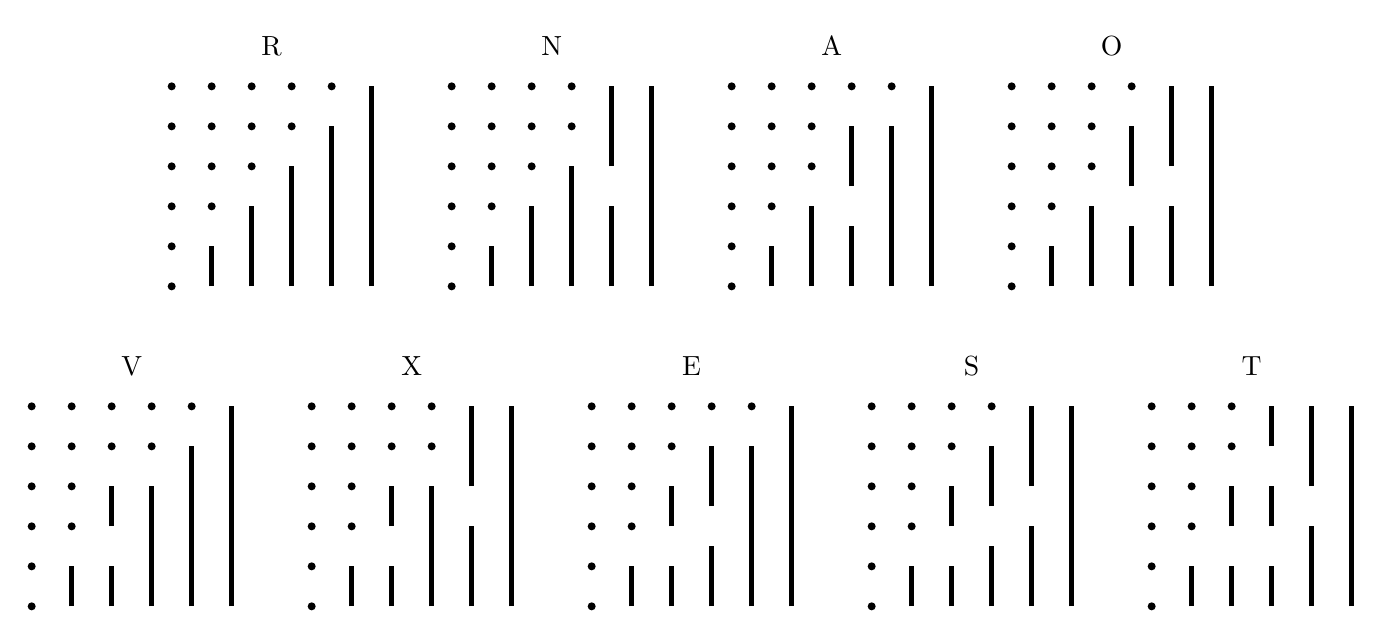
\begin{tikzpicture}[x=0.2in,y=0.2in]
\begin{scope}[shift={(3.5,0)}] 
\begin{scope}[shift={(0,0)}]
\fill[white] (0,0) rectangle (5,5);
\foreach \y in {0,1,2,3,4,5} {\fill (0,\y) circle (0.1);}
\foreach \y in {2,3,4,5} {\fill (1,\y) circle (0.1);}
\foreach \y in {3,4,5} {\fill (2,\y) circle (0.1);}
\foreach \y in {4,5} {\fill (3,\y) circle (0.1);}
\foreach \y in {5} {\fill (4,\y) circle (0.1);}
\draw[line width=2pt] (1,0) -- (1,1); 
\draw[line width=2pt] (2,0) -- (2,2); 
\draw[line width=2pt] (3,0) -- (3,3); 
\draw[line width=2pt] (4,0) -- (4,4); 
\draw[line width=2pt] (5,0) -- (5,5); 
\node at (2.5,6) {R};
\end{scope} 
\begin{scope}[shift={(7,0)}]
\fill[white] (0,0) rectangle (5,5);
\foreach \y in {0,1,2,3,4,5} {\fill (0,\y) circle (0.1);}
\foreach \y in {2,3,4,5} {\fill (1,\y) circle (0.1);}
\foreach \y in {3,4,5} {\fill (2,\y) circle (0.1);}
\foreach \y in {4,5} {\fill (3,\y) circle (0.1);}
\draw[line width=2pt] (1,0) -- (1,1); 
\draw[line width=2pt] (2,0) -- (2,2); 
\draw[line width=2pt] (3,0) -- (3,3); 
\draw[line width=2pt] (4,0) -- (4,2); \draw[line width=2pt] (4,3) -- (4,5); 
\draw[line width=2pt] (5,0) -- (5,5); 
\node at (2.5,6) {N};
\end{scope} 
\begin{scope}[shift={(14,0)}]
\fill[white] (0,0) rectangle (5,5);
\foreach \y in {0,1,2,3,4,5} {\fill (0,\y) circle (0.1);}
\foreach \y in {2,3,4,5} {\fill (1,\y) circle (0.1);}
\foreach \y in {3,4,5} {\fill (2,\y) circle (0.1);}
\foreach \y in {5} {\fill (3,\y) circle (0.1);}
\foreach \y in {5} {\fill (4,\y) circle (0.1);}
\draw[line width=2pt] (1,0) -- (1,1); 
\draw[line width=2pt] (2,0) -- (2,2); 
\draw[line width=2pt] (3,0) -- (3,1.5); \draw[line width=2pt] (3,2.5) -- (3,4); 
\draw[line width=2pt] (4,0) -- (4,4);
\draw[line width=2pt] (5,0) -- (5,5); 
\node at (2.5,6) {A};
\end{scope} 
\begin{scope}[shift={(21,0)}]
\fill[white] (0,0) rectangle (5,5);
\foreach \y in {0,1,2,3,4,5} {\fill (0,\y) circle (0.1);}
\foreach \y in {2,3,4,5} {\fill (1,\y) circle (0.1);}
\foreach \y in {3,4,5} {\fill (2,\y) circle (0.1);}
\foreach \y in {5} {\fill (3,\y) circle (0.1);}
\draw[line width=2pt] (1,0) -- (1,1); 
\draw[line width=2pt] (2,0) -- (2,2); 
\draw[line width=2pt] (3,0) -- (3,1.5); \draw[line width=2pt] (3,2.5) -- (3,4); 
\draw[line width=2pt] (4,0) -- (4,2); \draw[line width=2pt] (4,3) -- (4,5); 
\draw[line width=2pt] (5,0) -- (5,5); 
\node at (2.5,6) {O};
\end{scope} 
\end{scope} 
\begin{scope}[shift={(0,-8)}]
\fill[white] (0,0) rectangle (5,5);
\foreach \y in {0,1,2,3,4,5} {\fill (0,\y) circle (0.1);}
\foreach \y in {2,3,4,5} {\fill (1,\y) circle (0.1);}
\foreach \y in {4,5} {\fill (2,\y) circle (0.1);}
\foreach \y in {4,5} {\fill (3,\y) circle (0.1);}
\foreach \y in {5} {\fill (4,\y) circle (0.1);}
\draw[line width=2pt] (1,0) -- (1,1); 
\draw[line width=2pt] (2,0) -- (2,1); \draw[line width=2pt] (2,2) -- (2,3); 
\draw[line width=2pt] (3,0) -- (3,3);
\draw[line width=2pt] (4,0) -- (4,4);
\draw[line width=2pt] (5,0) -- (5,5); 
\node at (2.5,6) {V};
\end{scope} 
\begin{scope}[shift={(7,-8)}]
\fill[white] (0,0) rectangle (5,5);
\foreach \y in {0,1,2,3,4,5} {\fill (0,\y) circle (0.1);}
\foreach \y in {2,3,4,5} {\fill (1,\y) circle (0.1);}
\foreach \y in {4,5} {\fill (2,\y) circle (0.1);}
\foreach \y in {4,5} {\fill (3,\y) circle (0.1);}
\draw[line width=2pt] (1,0) -- (1,1); 
\draw[line width=2pt] (2,0) -- (2,1); \draw[line width=2pt] (2,2) -- (2,3); 
\draw[line width=2pt] (3,0) -- (3,3);
\draw[line width=2pt] (4,0) -- (4,2); \draw[line width=2pt] (4,3) -- (4,5); 
\draw[line width=2pt] (5,0) -- (5,5); 
\node at (2.5,6) {X};
\end{scope} 
\begin{scope}[shift={(14,-8)}]
\fill[white] (0,0) rectangle (5,5);
\foreach \y in {0,1,2,3,4,5} {\fill (0,\y) circle (0.1);}
\foreach \y in {2,3,4,5} {\fill (1,\y) circle (0.1);}
\foreach \y in {4,5} {\fill (2,\y) circle (0.1);}
\foreach \y in {5} {\fill (3,\y) circle (0.1);}
\foreach \y in {5} {\fill (4,\y) circle (0.1);}
\draw[line width=2pt] (1,0) -- (1,1); 
\draw[line width=2pt] (2,0) -- (2,1); \draw[line width=2pt] (2,2) -- (2,3); 
\draw[line width=2pt] (3,0) -- (3,1.5); \draw[line width=2pt] (3,2.5) -- (3,4);
\draw[line width=2pt] (4,0) -- (4,4);
\draw[line width=2pt] (5,0) -- (5,5); 
\node at (2.5,6) {E};
\end{scope} 
\begin{scope}[shift={(21,-8)}]
\fill[white] (0,0) rectangle (5,5);
\foreach \y in {0,1,2,3,4,5} {\fill (0,\y) circle (0.1);}
\foreach \y in {2,3,4,5} {\fill (1,\y) circle (0.1);}
\foreach \y in {4,5} {\fill (2,\y) circle (0.1);}
\foreach \y in {5} {\fill (3,\y) circle (0.1);}
\draw[line width=2pt] (1,0) -- (1,1); 
\draw[line width=2pt] (2,0) -- (2,1); \draw[line width=2pt] (2,2) -- (2,3); 
\draw[line width=2pt] (3,0) -- (3,1.5); \draw[line width=2pt] (3,2.5) -- (3,4);
\draw[line width=2pt] (4,0) -- (4,2); \draw[line width=2pt] (4,3) -- (4,5); 
\draw[line width=2pt] (5,0) -- (5,5); 
\node at (2.5,6) {S};
\end{scope} 
\begin{scope}[shift={(28,-8)}]
\fill[white] (0,0) rectangle (5,5);
\foreach \y in {0,1,2,3,4,5} {\fill (0,\y) circle (0.1);}
\foreach \y in {2,3,4,5} {\fill (1,\y) circle (0.1);}
\foreach \y in {4,5} {\fill (2,\y) circle (0.1);}
\draw[line width=2pt] (1,0) -- (1,1); 
\draw[line width=2pt] (2,0) -- (2,1); \draw[line width=2pt] (2,2) -- (2,3); 
\draw[line width=2pt] (3,0) -- (3,1); \draw[line width=2pt] (3,2) -- (3,3);
  \draw[line width=2pt] (3,4) -- (3,5);
\draw[line width=2pt] (4,0) -- (4,2); \draw[line width=2pt] (4,3) -- (4,5); 
\draw[line width=2pt] (5,0) -- (5,5); 
\node at (2.5,6) {T};
\end{scope} 
\end{tikzpicture}

\vspace{0.5in}

\texttt{02-45-49-60-67-85}%V
\hspace{2em}
\texttt{11-28-38-43-72-84}%O
\hspace{2em}
\texttt{14-27-31-42-62-87}%R

\vspace{1in}

\texttt{04-15-37-50-73-80}%T
\hspace{2em}
\texttt{03-32-45-65-90-92}%E
\hspace{2em}
\texttt{12-32-64-70-89-96}%X
\end{center}


  \phWorksheet{Solution}

  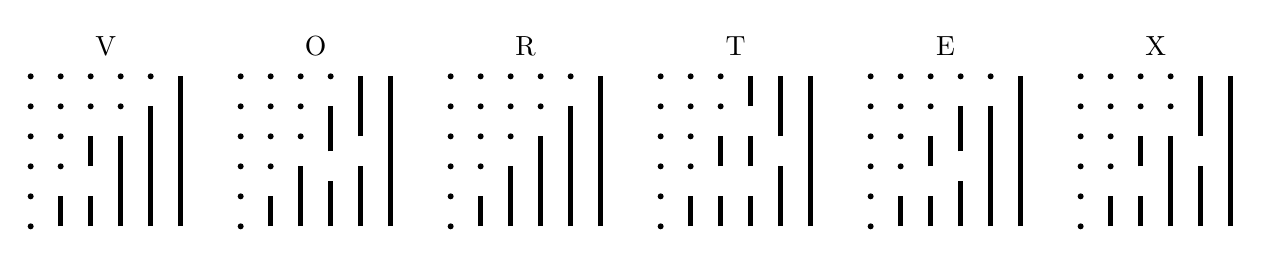
\begin{tikzpicture}[x=0.15in,y=0.15in]
\begin{scope}[shift={(14,0)}]
\fill[white] (0,0) rectangle (5,5);
\foreach \y in {0,1,2,3,4,5} {\fill (0,\y) circle (0.1);}
\foreach \y in {2,3,4,5} {\fill (1,\y) circle (0.1);}
\foreach \y in {3,4,5} {\fill (2,\y) circle (0.1);}
\foreach \y in {4,5} {\fill (3,\y) circle (0.1);}
\foreach \y in {5} {\fill (4,\y) circle (0.1);}
\draw[line width=2pt] (1,0) -- (1,1); 
\draw[line width=2pt] (2,0) -- (2,2); 
\draw[line width=2pt] (3,0) -- (3,3); 
\draw[line width=2pt] (4,0) -- (4,4); 
\draw[line width=2pt] (5,0) -- (5,5); 
\node at (2.5,6) {R};
\end{scope} 
\begin{scope}[shift={(7,0)}]
\fill[white] (0,0) rectangle (5,5);
\foreach \y in {0,1,2,3,4,5} {\fill (0,\y) circle (0.1);}
\foreach \y in {2,3,4,5} {\fill (1,\y) circle (0.1);}
\foreach \y in {3,4,5} {\fill (2,\y) circle (0.1);}
\foreach \y in {5} {\fill (3,\y) circle (0.1);}
\draw[line width=2pt] (1,0) -- (1,1); 
\draw[line width=2pt] (2,0) -- (2,2); 
\draw[line width=2pt] (3,0) -- (3,1.5); \draw[line width=2pt] (3,2.5) -- (3,4); 
\draw[line width=2pt] (4,0) -- (4,2); \draw[line width=2pt] (4,3) -- (4,5); 
\draw[line width=2pt] (5,0) -- (5,5); 
\node at (2.5,6) {O};
\end{scope} 
\begin{scope}[shift={(0,0)}]
\fill[white] (0,0) rectangle (5,5);
\foreach \y in {0,1,2,3,4,5} {\fill (0,\y) circle (0.1);}
\foreach \y in {2,3,4,5} {\fill (1,\y) circle (0.1);}
\foreach \y in {4,5} {\fill (2,\y) circle (0.1);}
\foreach \y in {4,5} {\fill (3,\y) circle (0.1);}
\foreach \y in {5} {\fill (4,\y) circle (0.1);}
\draw[line width=2pt] (1,0) -- (1,1); 
\draw[line width=2pt] (2,0) -- (2,1); \draw[line width=2pt] (2,2) -- (2,3); 
\draw[line width=2pt] (3,0) -- (3,3);
\draw[line width=2pt] (4,0) -- (4,4);
\draw[line width=2pt] (5,0) -- (5,5); 
\node at (2.5,6) {V};
\end{scope} 
\begin{scope}[shift={(35,0)}]
\fill[white] (0,0) rectangle (5,5);
\foreach \y in {0,1,2,3,4,5} {\fill (0,\y) circle (0.1);}
\foreach \y in {2,3,4,5} {\fill (1,\y) circle (0.1);}
\foreach \y in {4,5} {\fill (2,\y) circle (0.1);}
\foreach \y in {4,5} {\fill (3,\y) circle (0.1);}
\draw[line width=2pt] (1,0) -- (1,1); 
\draw[line width=2pt] (2,0) -- (2,1); \draw[line width=2pt] (2,2) -- (2,3); 
\draw[line width=2pt] (3,0) -- (3,3);
\draw[line width=2pt] (4,0) -- (4,2); \draw[line width=2pt] (4,3) -- (4,5); 
\draw[line width=2pt] (5,0) -- (5,5); 
\node at (2.5,6) {X};
\end{scope} 
\begin{scope}[shift={(28,0)}]
\fill[white] (0,0) rectangle (5,5);
\foreach \y in {0,1,2,3,4,5} {\fill (0,\y) circle (0.1);}
\foreach \y in {2,3,4,5} {\fill (1,\y) circle (0.1);}
\foreach \y in {4,5} {\fill (2,\y) circle (0.1);}
\foreach \y in {5} {\fill (3,\y) circle (0.1);}
\foreach \y in {5} {\fill (4,\y) circle (0.1);}
\draw[line width=2pt] (1,0) -- (1,1); 
\draw[line width=2pt] (2,0) -- (2,1); \draw[line width=2pt] (2,2) -- (2,3); 
\draw[line width=2pt] (3,0) -- (3,1.5); \draw[line width=2pt] (3,2.5) -- (3,4);
\draw[line width=2pt] (4,0) -- (4,4);
\draw[line width=2pt] (5,0) -- (5,5); 
\node at (2.5,6) {E};
\end{scope} 
\begin{scope}[shift={(21,0)}]
\fill[white] (0,0) rectangle (5,5);
\foreach \y in {0,1,2,3,4,5} {\fill (0,\y) circle (0.1);}
\foreach \y in {2,3,4,5} {\fill (1,\y) circle (0.1);}
\foreach \y in {4,5} {\fill (2,\y) circle (0.1);}
\draw[line width=2pt] (1,0) -- (1,1); 
\draw[line width=2pt] (2,0) -- (2,1); \draw[line width=2pt] (2,2) -- (2,3); 
\draw[line width=2pt] (3,0) -- (3,1); \draw[line width=2pt] (3,2) -- (3,3);
  \draw[line width=2pt] (3,4) -- (3,5);
\draw[line width=2pt] (4,0) -- (4,2); \draw[line width=2pt] (4,3) -- (4,5); 
\draw[line width=2pt] (5,0) -- (5,5); 
\node at (2.5,6) {T};
\end{scope} 
\end{tikzpicture}


\phChapterWorksheet{Jumping Through Hyperspace}{Main Puzzle 4}

  On this system, your adventure takes you to a raucous space saloon, swapping tales
with Jan Duet, an infamous smuggler with a heart of gold.

She explains to you that in the early days of hyperspace travel, engines could
instantly transport ships between only certain locations on a six-lightyear continuum.
These options were illustrated using a graph, where the horizontal coordinate
represents starting positions, and the vertical coordinate represents ending positions.

%In Example A illustrated below, a ship at position \(0\) could be teleported
%to any position between \(0\) and \(6\), a ship at position \(0.5\) could only
%be teleported to positions \(4.5\) or \(6\), and a ship at any position between
%\(2\) and \(6\) could only be teleported to position \(6\).

The goal of a hyperspace engine is to be ``ideal'': the collection of possible
destinations from any particular point using exactly one teleportation should be exactly the 
same as the collection of possible destinations that can
be reached from that point using exactly two teleportations.

This means Example A is not ideal. Position \(1\) teleports to
positions \(5\) and \(6\), but from positions \(5\) and \(6\), there are two
problems: a new destination \(3\) can be reached, and the destination \(5\) can
no longer be reached.

However, Example B is ideal. From \(0\), any position can be reached after either
one or two teleportations. From \(2\), positions \(3\) and \(6\) can be reached
after either one or two teleportations. From \(4\), only position \(6\) can be reached
after one or two teleportations. From \(5\), positions \(5\) and \(6\) can be
reached after one or two teleportations. And so on (even for fractional positions!).

Jan suggests that you review your \textbf{Hyperspace Engines} document;
perhaps the illustrations representing ideal engines will reveal a hidden codeword?

\begin{center}
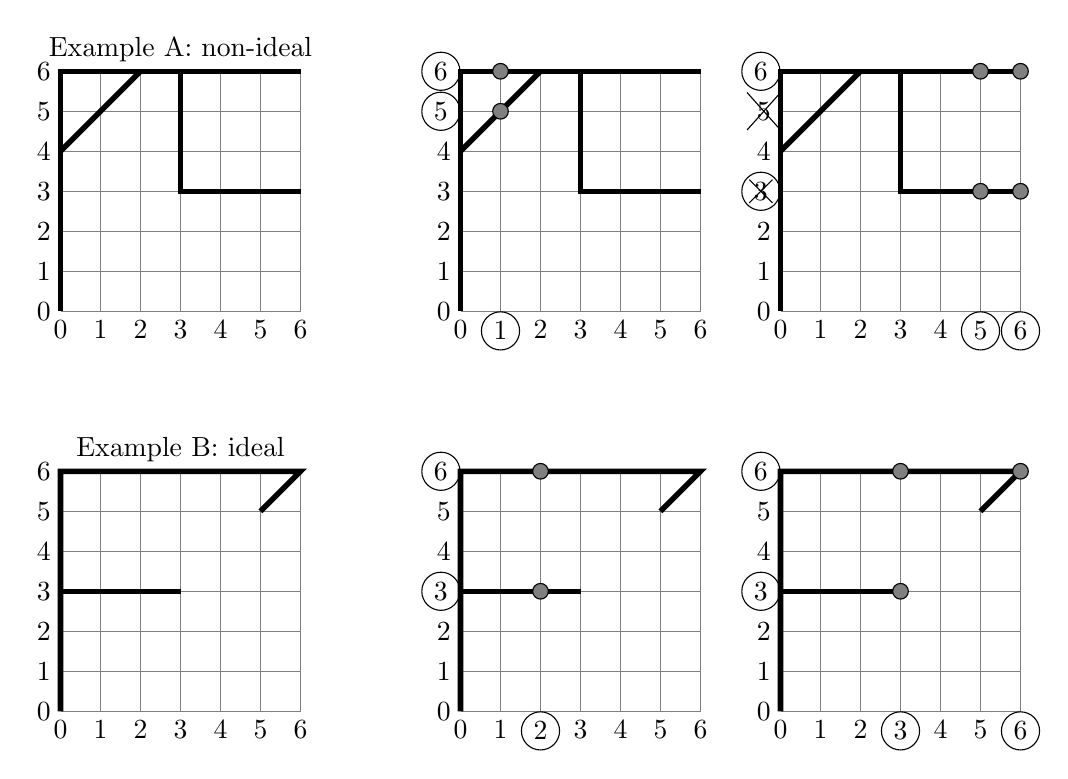
\begin{tikzpicture}[x=0.2in,y=0.2in] 
\begin{scope}[shift={(0,0)}] 
\node[anchor=south] at (3,6) {Example A: non-ideal};
\fill[white] (0,0) rectangle (6,6);
\draw[step=1,thin,gray] (0,0) grid (6,6);
\draw[line width=2pt] (0,0) -- (0,6) -- (6,6);
\draw[line width=2pt] (0,4) -- (2,6);
\draw[line width=2pt] (3,6) -- (3,3) -- (6,3);
\foreach \x in {0,1,2,3,4,5,6} {
  \node[anchor=north] at (\x,0) {\(\x\)};
}
\foreach \y in {0,1,2,3,4,5,6} {
  \node[anchor=east] at (0,\y) {\(\y\)};
}
\end{scope}
\begin{scope}[shift={(10,0)}] 
\fill[white] (0,0) rectangle (6,6);
\draw[step=1,thin,gray] (0,0) grid (6,6);
\draw[line width=2pt] (0,0) -- (0,6) -- (6,6);
\draw[line width=2pt] (0,4) -- (2,6);
\draw[line width=2pt] (3,6) -- (3,3) -- (6,3);
\foreach \x in {0,2,3,4,5,6} {
  \node[anchor=north] at (\x,0) {\(\x\)};
}
\foreach \y in {0,1,2,3,4} {
  \node[anchor=east] at (0,\y) {\(\y\)};
}
\node[anchor=north,draw,inner sep=2pt,shape=circle] at (1,0) {\(1\)};
\node[anchor=east,draw,inner sep=2pt,shape=circle] at (0,5) {\(5\)};
\node[anchor=east,draw,inner sep=2pt,shape=circle] at (0,6) {\(6\)};
\node[fill=gray,draw,inner sep=2pt,shape=circle] at (1,5) {};
\node[fill=gray,draw,inner sep=2pt,shape=circle] at (1,6) {};
\end{scope}
\begin{scope}[shift={(18,0)}] 
\fill[white] (0,0) rectangle (6,6);
\draw[step=1,thin,gray] (0,0) grid (6,6);
\draw[line width=2pt] (0,0) -- (0,6) -- (6,6);
\draw[line width=2pt] (0,4) -- (2,6);
\draw[line width=2pt] (3,6) -- (3,3) -- (6,3);
\foreach \x in {0,1,2,3,4} {
  \node[anchor=north] at (\x,0) {\(\x\)};
}
\foreach \y in {0,1,2,4} {
  \node[anchor=east] at (0,\y) {\(\y\)};
}
\node[anchor=north,draw,inner sep=2pt,shape=circle] at (5,0) {\(5\)};
\node[anchor=north,draw,inner sep=2pt,shape=circle] at (6,0) {\(6\)};
\node[anchor=east,draw,cross out] at (0,5) {\(5\)};
\node[anchor=east,draw,inner sep=2pt,shape=circle] at (0,6) {\(6\)};
\node[anchor=east,draw,inner sep=2pt,shape=circle] at (0,3) {\(3\)};
\node[anchor=east,draw,inner sep=4pt,cross out] at (-0.2,3) {};
\node[fill=gray,draw,inner sep=2pt,shape=circle] at (5,6) {};
\node[fill=gray,draw,inner sep=2pt,shape=circle] at (6,6) {};
\node[fill=gray,draw,inner sep=2pt,shape=circle] at (5,3) {};
\node[fill=gray,draw,inner sep=2pt,shape=circle] at (6,3) {};
\end{scope}

\begin{scope}[shift={(0,-10)}] 
\node[anchor=south] at (3,6) {Example B: ideal};
\fill[white] (0,0) rectangle (6,6);
\draw[step=1,thin,gray] (0,0) grid (6,6);
\draw[line width=2pt] (0,0) -- (0,6) -- (6,6) -- (5,5);
\draw[line width=2pt] (0,3) -- (3,3);
\foreach \x in {0,1,2,3,4,5,6} {
  \node[anchor=north] at (\x,0) {\(\x\)};
}
\foreach \y in {0,1,2,3,4,5,6} {
  \node[anchor=east] at (0,\y) {\(\y\)};
}
\end{scope}
\begin{scope}[shift={(10,-10)}] 
\fill[white] (0,0) rectangle (6,6);
\draw[step=1,thin,gray] (0,0) grid (6,6);
\draw[line width=2pt] (0,0) -- (0,6) -- (6,6) -- (5,5);
\draw[line width=2pt] (0,3) -- (3,3);
\foreach \x in {0,1,3,4,5,6} {
  \node[anchor=north] at (\x,0) {\(\x\)};
}
\foreach \y in {0,1,2,4,5} {
  \node[anchor=east] at (0,\y) {\(\y\)};
}
\node[anchor=north,draw,inner sep=2pt,shape=circle] at (2,0) {\(2\)};
\node[anchor=east,draw,inner sep=2pt,shape=circle] at (0,3) {\(3\)};
\node[anchor=east,draw,inner sep=2pt,shape=circle] at (0,6) {\(6\)};
\node[fill=gray,draw,inner sep=2pt,shape=circle] at (2,3) {};
\node[fill=gray,draw,inner sep=2pt,shape=circle] at (2,6) {};
\end{scope}
\begin{scope}[shift={(18,-10)}] 
\fill[white] (0,0) rectangle (6,6);
\draw[step=1,thin,gray] (0,0) grid (6,6);
\draw[line width=2pt] (0,0) -- (0,6) -- (6,6) -- (5,5);
\draw[line width=2pt] (0,3) -- (3,3);
\foreach \x in {0,1,2,4,5} {
  \node[anchor=north] at (\x,0) {\(\x\)};
}
\foreach \y in {0,1,2,4,5} {
  \node[anchor=east] at (0,\y) {\(\y\)};
}
\node[anchor=north,draw,inner sep=2pt,shape=circle] at (3,0) {\(3\)};
\node[anchor=north,draw,inner sep=2pt,shape=circle] at (6,0) {\(6\)};
\node[anchor=east,draw,inner sep=2pt,shape=circle] at (0,3) {\(3\)};
\node[anchor=east,draw,inner sep=2pt,shape=circle] at (0,6) {\(6\)};
\node[fill=gray,draw,inner sep=2pt,shape=circle] at (3,3) {};
\node[fill=gray,draw,inner sep=2pt,shape=circle] at (3,6) {};
\node[fill=gray,draw,inner sep=2pt,shape=circle] at (6,6) {};
\end{scope}
\end{tikzpicture}
\end{center}

 


  \phWorksheet{Hyperspace Engines}

  \begin{center}
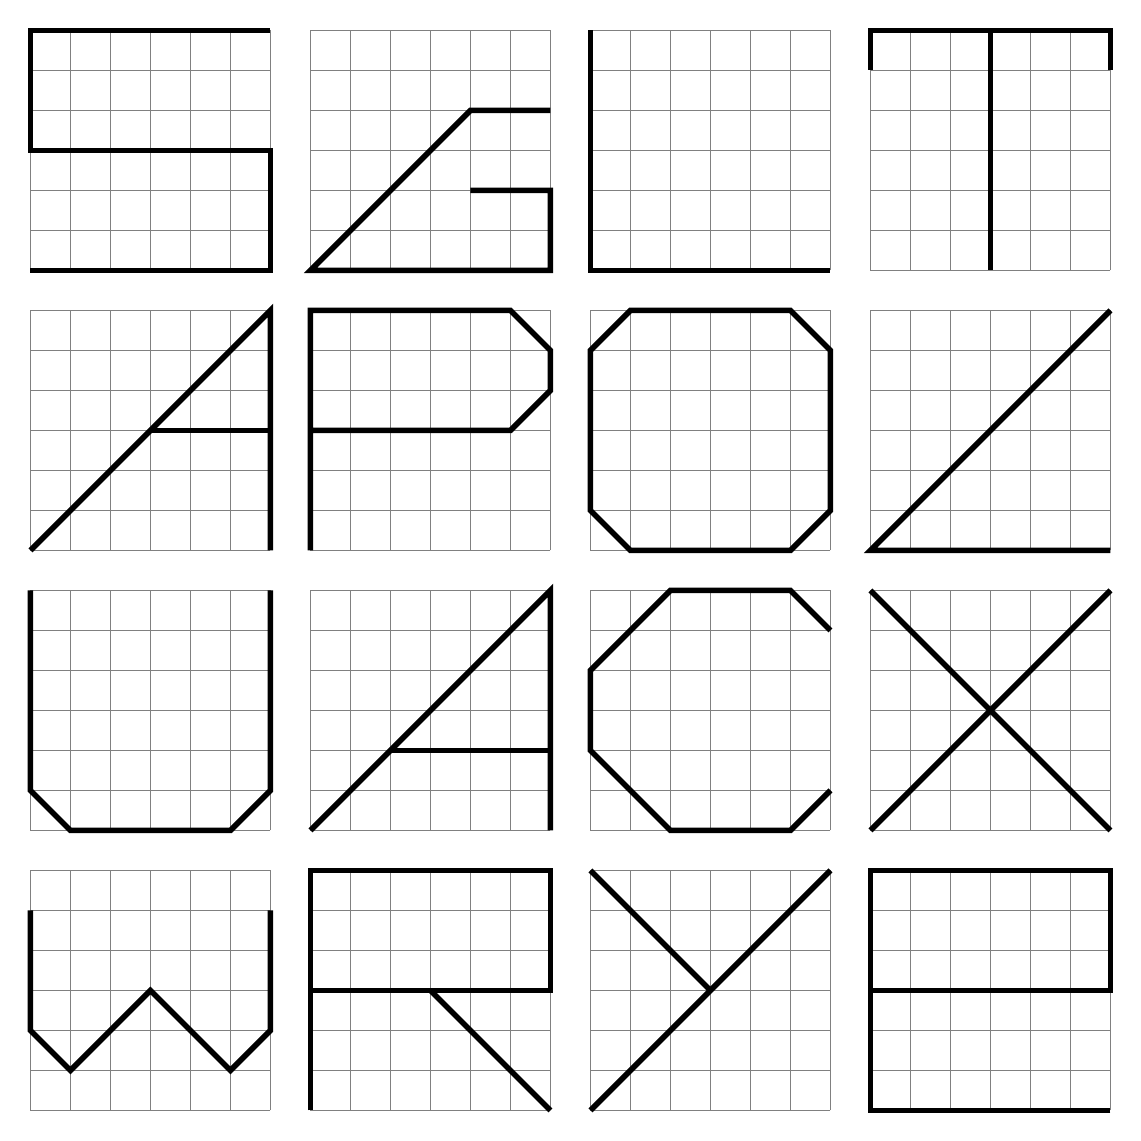
\begin{tikzpicture}[x=0.2in,y=0.2in] 
\begin{scope}[shift={(0,21)}] %BAD S
\fill[white] (0,0) rectangle (6,6);
\draw[step=1,thin,gray] (0,0) grid (6,6);
\draw[line width=2pt] (6,6) -- (0,6) -- (0,3) -- (6,3) -- (6,0) -- (0,0); 
\end{scope} 
\begin{scope}[shift={(7,21)}] %GOOD G
\fill[white] (0,0) rectangle (6,6);
\draw[step=1,thin,gray] (0,0) grid (6,6);
\draw[line width=2pt] (4,2) -- (6,2) -- (6,0) -- (0,0) -- (4,4) -- (6,4);
\end{scope}
\begin{scope}[shift={(14,21)}] %BAD L
\fill[white] (0,0) rectangle (6,6);
\draw[step=1,thin,gray] (0,0) grid (6,6);
\draw[line width=2pt] (0,6) -- (0,0) -- (6,0); 
\end{scope}
\begin{scope}[shift={(21,21)}] %BAD T
\fill[white] (0,0) rectangle (6,6);
\draw[step=1,thin,gray] (0,0) grid (6,6);
\draw[line width=2pt] (6,5) -- (6,6) -- (0,6) -- (0,5);
\draw[line width=2pt] (3,6) -- (3,0);
\end{scope}

\begin{scope}[shift={(0,14)}] %GOOD A(1)
\fill[white] (0,0) rectangle (6,6);
\draw[step=1,thin,gray] (0,0) grid (6,6);
\draw[line width=2pt] (0,0) -- (6,6) -- (6,0);
\draw[line width=2pt] (3,3) -- (6,3);
\end{scope}
\begin{scope}[shift={(7,14)}] %BAD P
\fill[white] (0,0) rectangle (6,6);
\draw[step=1,thin,gray] (0,0) grid (6,6);
\draw[line width=2pt] (0,0) -- (0,6) -- (5,6) -- (6,5) -- (6,4) -- (5,3) -- (0,3);
\end{scope}
\begin{scope}[shift={(14,14)}] %BAD O
\fill[white] (0,0) rectangle (6,6);
\draw[step=1,thin,gray] (0,0) grid (6,6);
\draw[line width=2pt] (0,1) -- (0,5) -- (1,6) -- (5,6) -- (6,5) -- (6,1) -- (5,0) -- (1,0) -- cycle; 
\end{scope}
\begin{scope}[shift={(21,14)}] %GOOD L
\fill[white] (0,0) rectangle (6,6);
\draw[step=1,thin,gray] (0,0) grid (6,6);
\draw[line width=2pt] (6,0) -- (0,0) -- (6,6);
\end{scope}

\begin{scope}[shift={(0,7)}] %BAD U
\fill[white] (0,0) rectangle (6,6);
\draw[step=1,thin,gray] (0,0) grid (6,6);
\draw[line width=2pt] (0,6) -- (0,1) -- (1,0) -- (5,0) -- (6,1) -- (6,6);
\end{scope}
\begin{scope}[shift={(7,7)}] %GOOD A(2)
\fill[white] (0,0) rectangle (6,6);
\draw[step=1,thin,gray] (0,0) grid (6,6);
\draw[line width=2pt] (0,0) -- (6,6) -- (6,0);
\draw[line width=2pt] (2,2) -- (6,2);
\end{scope}
\begin{scope}[shift={(14,7)}] %BAD C
\fill[white] (0,0) rectangle (6,6);
\draw[step=1,thin,gray] (0,0) grid (6,6);
\draw[line width=2pt] (6,1) -- (5,0) -- (2,0) -- (0,2) -- (0,4) -- (2,6) -- (5,6) -- (6,5); 
\end{scope}
\begin{scope}[shift={(21,7)}] %GOOD X
\fill[white] (0,0) rectangle (6,6);
\draw[step=1,thin,gray] (0,0) grid (6,6);
\draw[line width=2pt] (0,0) -- (6,6);
\draw[line width=2pt] (0,6) -- (6,0);
\end{scope}

\begin{scope}[shift={(0,0)}] %BAD W
\fill[white] (0,0) rectangle (6,6);
\draw[step=1,thin,gray] (0,0) grid (6,6);
\draw[line width=2pt] (0,5) -- (0,2) -- (1,1) -- (3,3) -- (5,1) -- (6,2) -- (6,5);
\end{scope}
\begin{scope}[shift={(7,0)}] %BAD R
\fill[white] (0,0) rectangle (6,6);
\draw[step=1,thin,gray] (0,0) grid (6,6);
\draw[line width=2pt] (0,0) -- (0,6) -- (6,6) -- (6,3) -- (0,3); 
\draw[line width=2pt] (3,3) -- (6,0);
\end{scope}
\begin{scope}[shift={(14,0)}] %GOOD Y
\fill[white] (0,0) rectangle (6,6);
\draw[step=1,thin,gray] (0,0) grid (6,6);
\draw[line width=2pt] (0,0) -- (6,6);
\draw[line width=2pt] (0,6) -- (3,3);
\end{scope}
\begin{scope}[shift={(21,0)}] %BAD E
\fill[white] (0,0) rectangle (6,6);
\draw[step=1,thin,gray] (0,0) grid (6,6);
\draw[line width=2pt] (6,0) -- (0,0) -- (0,6) -- (6,6) -- (6,3) -- (0,3);
\end{scope}
\end{tikzpicture}
\end{center}


\phChapterWorksheet{Out of Gas}{Cryptic Puzzle 2}

  Uh-oh... unforunately, you have now found yourself stranded
in a stretch of empty space with no fuel left! Maybe these firefly-class
engines aren't all they're cracked up to be...

Luckily for you,
your ship's \textit{amazing} engineer Faylee does have one trick that
just might save your team. There is
an emergency reserve tank that can be unlocked by utilizing the
\textbf{Reserve Tank Switchboard}, if you can puzzle out the meaning
of the following image...

\begin{center}
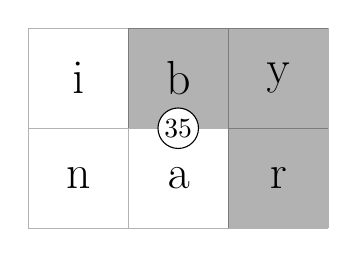
\begin{tikzpicture}[x=0.5in,y=0.5in]
\fill[white] (0,0) rectangle (3,2);
\draw[step=1,black!30] (0,0) grid (3,2);
\node at (1.5,1.5) {\LARGE b};
\node at (0.5,1.5) {\LARGE i};
\node at (0.5,0.5) {\LARGE n};
\node at (1.5,0.5) {\LARGE a};
\node at (2.5,0.5) {\LARGE r};
\node at (2.5,1.5) {\LARGE y};
\foreach \coor in {
  {(2,0)},
  {(1,1)},
  {(2,1)}
}{ \fill[opacity=0.3] \coor rectangle +(1,1); }
\node[circle,draw=black,fill=white,inner sep=1pt] at (1.5,1) {35};
\end{tikzpicture}
\end{center} 


  \phWorksheet{Reserve Tank Switchboard}

  \begin{center}
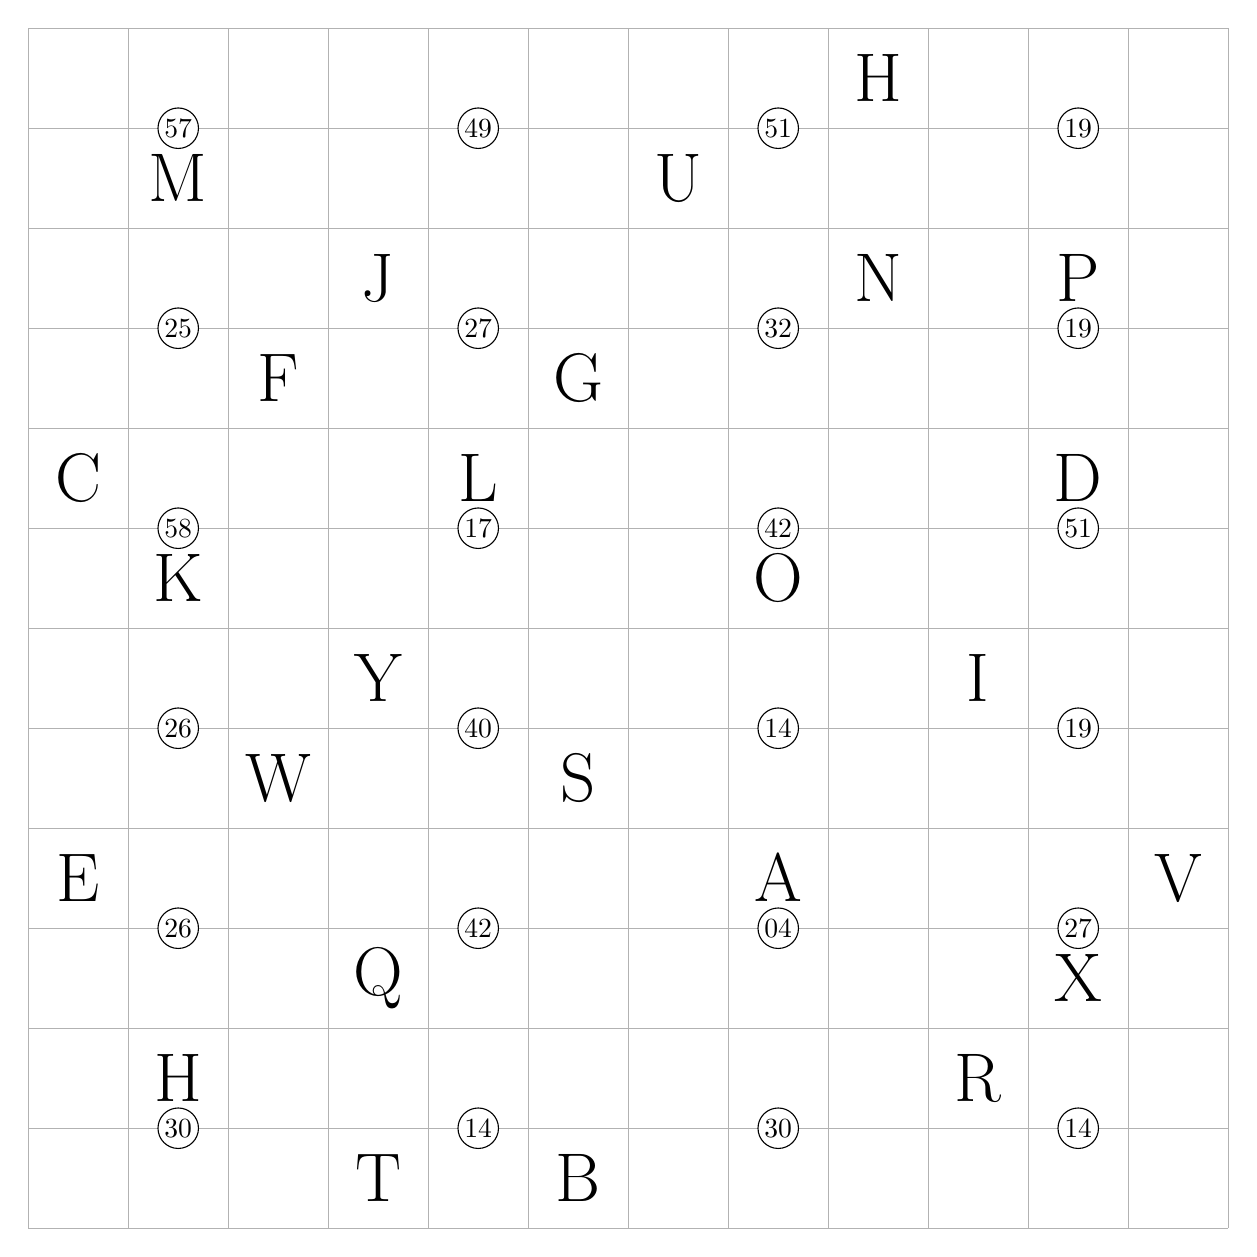
\begin{tikzpicture}[x=0.5in,y=0.5in]
\fill[white] (0,0) rectangle (12,12);
\draw[step=1,black!30] (0,0) grid (12,12);
\node at (10.5,9.5) {\Huge P};
\node at (6.5,10.5) {\Huge U};
\node at (4.5,7.5) {\Huge L};
\node at (5.5,4.5) {\Huge S};
\node at (7.5,3.5) {\Huge A};
\node at (9.5,1.5) {\Huge R};
% distractors
\node at (3.5,0.5) {\Huge T};
\node at (5.5,0.5) {\Huge B};
\node at (1.5,1.5) {\Huge H};
\node at (3.5,2.5) {\Huge Q};
\node at (10.5,2.5) {\Huge X};
\node at (0.5,3.5) {\Huge E};
\node at (11.5,3.5) {\Huge V};
\node at (2.5,4.5) {\Huge W};
\node at (3.5,5.5) {\Huge Y};
\node at (9.5,5.5) {\Huge I};
\node at (1.5,6.5) {\Huge K};
\node at (7.5,6.5) {\Huge O};
\node at (0.5,7.5) {\Huge C};
\node at (10.5,7.5) {\Huge D};
\node at (2.5,8.5) {\Huge F};
\node at (5.5,8.5) {\Huge G};
\node at (8.5,9.5) {\Huge N};
\node at (8.5,11.5) {\Huge H};
\node at (3.5,9.5) {\Huge J};
\node at (1.5,10.5) {\Huge M};
%numbers
\node[circle,draw=black,fill=white,inner sep=1pt] at (1.5,11) {57};
\node[circle,draw=black,fill=white,inner sep=1pt] at (4.5,11) {49};
\node[circle,draw=black,fill=white,inner sep=1pt] at (7.5,11) {51};
\node[circle,draw=black,fill=white,inner sep=1pt] at (10.5,11) {19};
\node[circle,draw=black,fill=white,inner sep=1pt] at (1.5,9) {25};
\node[circle,draw=black,fill=white,inner sep=1pt] at (4.5,9) {27};
\node[circle,draw=black,fill=white,inner sep=1pt] at (7.5,9) {32};
\node[circle,draw=black,fill=white,inner sep=1pt] at (10.5,9) {19};
\node[circle,draw=black,fill=white,inner sep=1pt] at (1.5,7) {58};
\node[circle,draw=black,fill=white,inner sep=1pt] at (4.5,7) {17};
\node[circle,draw=black,fill=white,inner sep=1pt] at (7.5,7) {42};
\node[circle,draw=black,fill=white,inner sep=1pt] at (10.5,7) {51};
\node[circle,draw=black,fill=white,inner sep=1pt] at (1.5,5) {26};
\node[circle,draw=black,fill=white,inner sep=1pt] at (4.5,5) {40};
\node[circle,draw=black,fill=white,inner sep=1pt] at (7.5,5) {14};
\node[circle,draw=black,fill=white,inner sep=1pt] at (10.5,5) {19};
\node[circle,draw=black,fill=white,inner sep=1pt] at (1.5,3) {26};
\node[circle,draw=black,fill=white,inner sep=1pt] at (4.5,3) {42};
\node[circle,draw=black,fill=white,inner sep=1pt] at (7.5,3) {04};
\node[circle,draw=black,fill=white,inner sep=1pt] at (10.5,3) {27};
\node[circle,draw=black,fill=white,inner sep=1pt] at (1.5,1) {30};
\node[circle,draw=black,fill=white,inner sep=1pt] at (4.5,1) {14};
\node[circle,draw=black,fill=white,inner sep=1pt] at (7.5,1) {30};
\node[circle,draw=black,fill=white,inner sep=1pt] at (10.5,1) {14};
% solution
%\foreach \coor in {
%  {(0,0)},
%  {(1,0)},
%  {(2,0)},
%  {(3,0)},
%  {(4,0)},
%  {(5,0)},
%  {(6,0)},
%  {(7,0)},
%  {(8,0)},
%  {(9,0)},
%  {(10,0)},
%  {(11,0)},
%  {(0,1)},
%  {(6,1)},
%  {(0,2)},
%  {(2,2)},
%  {(3,2)},
%  {(5,2)},
%  {(7,2)},
%  {(9,2)},
%  {(11,2)},
%  {(0,3)},
%  {(4,3)},
%  {(9,3)},
%  {(11,3)},
%  {(0,4)},
%  {(2,4)},
%  {(3,4)},
%  {(6,4)},
%  {(7,4)},
%  {(8,4)},
%  {(11,4)},
%  {(0,5)},
%  {(4,5)},
%  {(9,5)},
%  {(11,5)},
%  {(0,6)},
%  {(2,6)},
%  {(6,6)},
%  {(8,6)},
%  {(11,6)},
%  {(0,7)},
%  {(1,7)},
%  {(3,7)},
%  {(5,7)},
%  {(7,7)},
%  {(9,7)},
%  {(10,7)},
%  {(11,7)},
%  {(0,8)},
%  {(3,8)},
%  {(5,8)},
%  {(11,8)},
%  {(0,9)},
%  {(2,9)},
%  {(3,9)},
%  {(5,9)},
%  {(7,9)},
%  {(9,9)},
%  {(11,9)},
%  {(0,10)},
%  {(8,10)},
%  {(11,10)},
%  {(0,11)},
%  {(1,11)},
%  {(2,11)},
%  {(3,11)},
%  {(4,11)},
%  {(5,11)},
%  {(6,11)},
%  {(7,11)},
%  {(8,11)},
%  {(9,11)},
%  {(11,11)}
%}{ \fill[opacity=0.5] \coor rectangle +(1,1); }
%\draw[red] 
%  (10.5,12.5) -- 
%  (10.5,8.5) --
%  (6.5,8.5) --
%  (6.5,10.5) --
%  (4.5,10.5) --
%  (4.5,6.5) --
%  (5.5,6.5) --
%  (5.5,3.5) --
%  (8.5,3.5) --
%  (8.5,1.5) --
%  (12.5,1.5);
\end{tikzpicture}
\end{center}


  \phWorksheet{Solution}

  Using binary to fill in the grid as in the attachment,
a maze is revealed.

\begin{center}
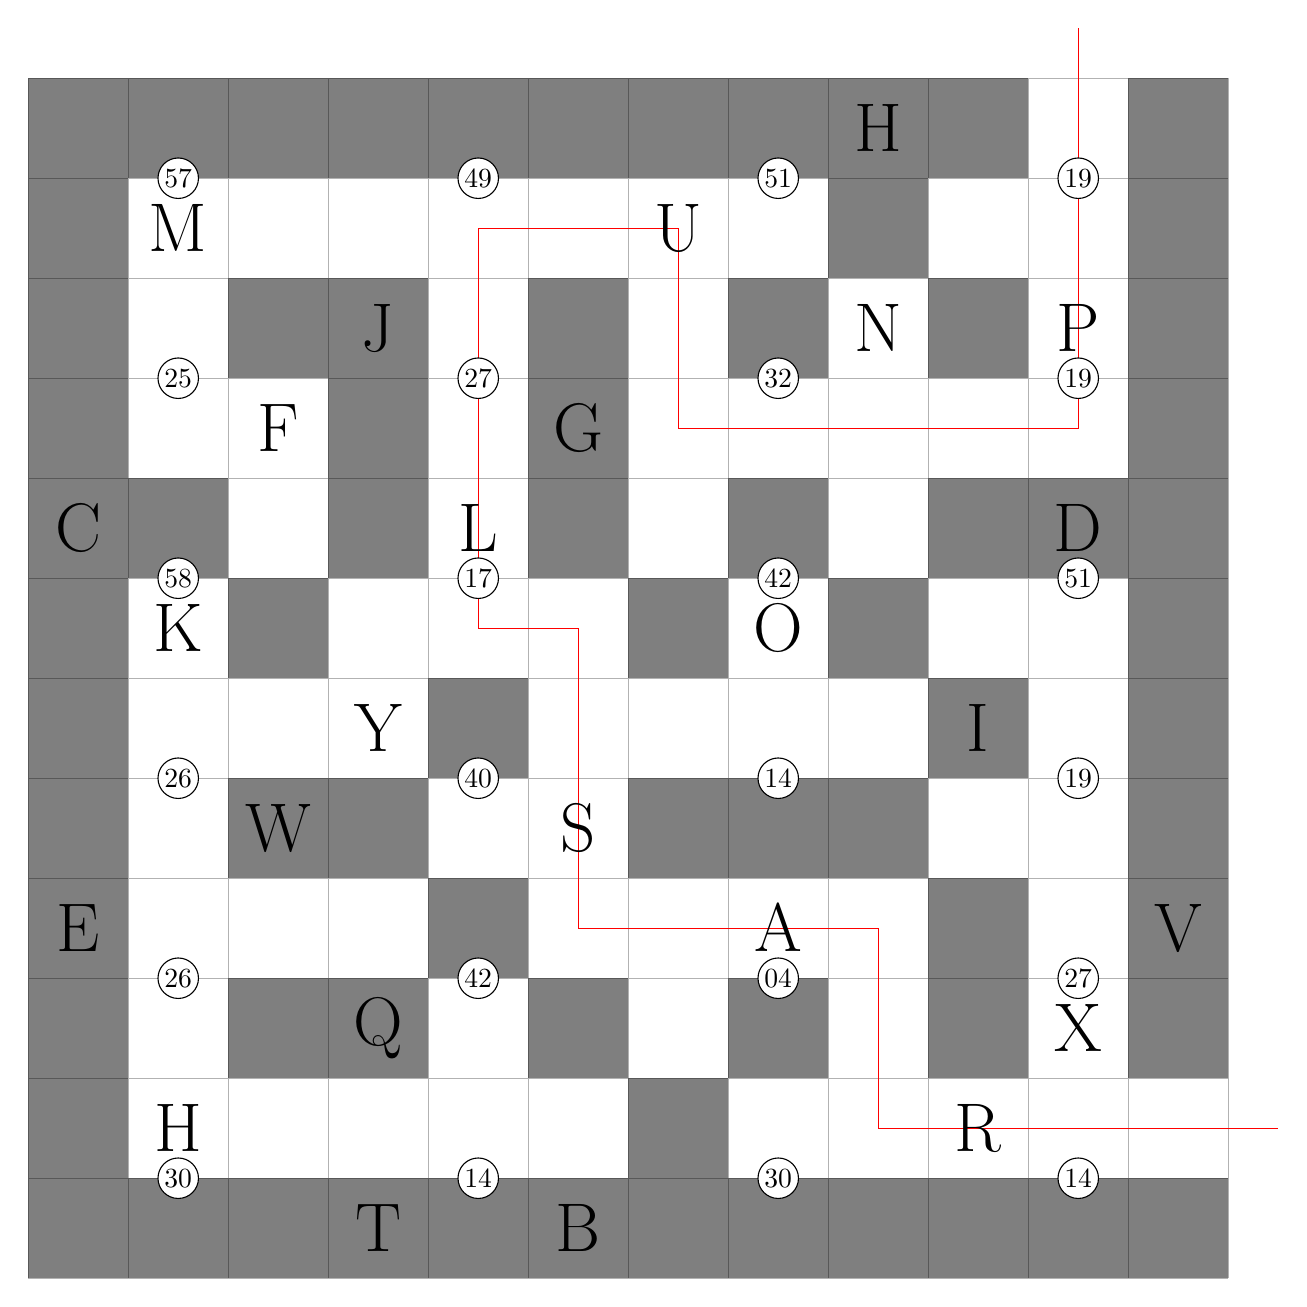
\begin{tikzpicture}[x=0.5in,y=0.5in]
\fill[white] (0,0) rectangle (12,12);
\draw[step=1,black!30] (0,0) grid (12,12);
% solution
\foreach \coor in {
  {(0,0)},
  {(1,0)},
  {(2,0)},
  {(3,0)},
  {(4,0)},
  {(5,0)},
  {(6,0)},
  {(7,0)},
  {(8,0)},
  {(9,0)},
  {(10,0)},
  {(11,0)},
  {(0,1)},
  {(6,1)},
  {(0,2)},
  {(2,2)},
  {(3,2)},
  {(5,2)},
  {(7,2)},
  {(9,2)},
  {(11,2)},
  {(0,3)},
  {(4,3)},
  {(9,3)},
  {(11,3)},
  {(0,4)},
  {(2,4)},
  {(3,4)},
  {(6,4)},
  {(7,4)},
  {(8,4)},
  {(11,4)},
  {(0,5)},
  {(4,5)},
  {(9,5)},
  {(11,5)},
  {(0,6)},
  {(2,6)},
  {(6,6)},
  {(8,6)},
  {(11,6)},
  {(0,7)},
  {(1,7)},
  {(3,7)},
  {(5,7)},
  {(7,7)},
  {(9,7)},
  {(10,7)},
  {(11,7)},
  {(0,8)},
  {(3,8)},
  {(5,8)},
  {(11,8)},
  {(0,9)},
  {(2,9)},
  {(3,9)},
  {(5,9)},
  {(7,9)},
  {(9,9)},
  {(11,9)},
  {(0,10)},
  {(8,10)},
  {(11,10)},
  {(0,11)},
  {(1,11)},
  {(2,11)},
  {(3,11)},
  {(4,11)},
  {(5,11)},
  {(6,11)},
  {(7,11)},
  {(8,11)},
  {(9,11)},
  {(11,11)}
}{ \fill[opacity=0.5] \coor rectangle +(1,1); }
\draw[red] 
  (10.5,12.5) -- 
  (10.5,8.5) --
  (6.5,8.5) --
  (6.5,10.5) --
  (4.5,10.5) --
  (4.5,6.5) --
  (5.5,6.5) --
  (5.5,3.5) --
  (8.5,3.5) --
  (8.5,1.5) --
  (12.5,1.5);
\node at (10.5,9.5) {\Huge P};
\node at (6.5,10.5) {\Huge U};
\node at (4.5,7.5) {\Huge L};
\node at (5.5,4.5) {\Huge S};
\node at (7.5,3.5) {\Huge A};
\node at (9.5,1.5) {\Huge R};
% distractors
\node at (3.5,0.5) {\Huge T};
\node at (5.5,0.5) {\Huge B};
\node at (1.5,1.5) {\Huge H};
\node at (3.5,2.5) {\Huge Q};
\node at (10.5,2.5) {\Huge X};
\node at (0.5,3.5) {\Huge E};
\node at (11.5,3.5) {\Huge V};
\node at (2.5,4.5) {\Huge W};
\node at (3.5,5.5) {\Huge Y};
\node at (9.5,5.5) {\Huge I};
\node at (1.5,6.5) {\Huge K};
\node at (7.5,6.5) {\Huge O};
\node at (0.5,7.5) {\Huge C};
\node at (10.5,7.5) {\Huge D};
\node at (2.5,8.5) {\Huge F};
\node at (5.5,8.5) {\Huge G};
\node at (8.5,9.5) {\Huge N};
\node at (8.5,11.5) {\Huge H};
\node at (3.5,9.5) {\Huge J};
\node at (1.5,10.5) {\Huge M};
%numbers
\node[circle,draw=black,fill=white,inner sep=1pt] at (1.5,11) {57};
\node[circle,draw=black,fill=white,inner sep=1pt] at (4.5,11) {49};
\node[circle,draw=black,fill=white,inner sep=1pt] at (7.5,11) {51};
\node[circle,draw=black,fill=white,inner sep=1pt] at (10.5,11) {19};
\node[circle,draw=black,fill=white,inner sep=1pt] at (1.5,9) {25};
\node[circle,draw=black,fill=white,inner sep=1pt] at (4.5,9) {27};
\node[circle,draw=black,fill=white,inner sep=1pt] at (7.5,9) {32};
\node[circle,draw=black,fill=white,inner sep=1pt] at (10.5,9) {19};
\node[circle,draw=black,fill=white,inner sep=1pt] at (1.5,7) {58};
\node[circle,draw=black,fill=white,inner sep=1pt] at (4.5,7) {17};
\node[circle,draw=black,fill=white,inner sep=1pt] at (7.5,7) {42};
\node[circle,draw=black,fill=white,inner sep=1pt] at (10.5,7) {51};
\node[circle,draw=black,fill=white,inner sep=1pt] at (1.5,5) {26};
\node[circle,draw=black,fill=white,inner sep=1pt] at (4.5,5) {40};
\node[circle,draw=black,fill=white,inner sep=1pt] at (7.5,5) {14};
\node[circle,draw=black,fill=white,inner sep=1pt] at (10.5,5) {19};
\node[circle,draw=black,fill=white,inner sep=1pt] at (1.5,3) {26};
\node[circle,draw=black,fill=white,inner sep=1pt] at (4.5,3) {42};
\node[circle,draw=black,fill=white,inner sep=1pt] at (7.5,3) {04};
\node[circle,draw=black,fill=white,inner sep=1pt] at (10.5,3) {27};
\node[circle,draw=black,fill=white,inner sep=1pt] at (1.5,1) {30};
\node[circle,draw=black,fill=white,inner sep=1pt] at (4.5,1) {14};
\node[circle,draw=black,fill=white,inner sep=1pt] at (7.5,1) {30};
\node[circle,draw=black,fill=white,inner sep=1pt] at (10.5,1) {14};
\end{tikzpicture}
\end{center}

The solution is the letters appearing on the unique solution to the maze:
\texttt{PULSAR}


\phChapterWorksheet{Word Problem}{Cryptic Puzzle 4}

  As your adventures continue, your ship comes across a \textbf{Myserious
Message}, projected onto the stars themselves! You put on a John
Williams soundtrack, but to no avail, as the strange communication
frankly doesn't make any sense. It's as though nine of the
words don't belong...

You contact Jan Duet, who says this isn't the first time she's
come across such a message. She suggests that while she's gone
to great \textit{lengths} to decipher the true meaning of
these dispatches, she always ends up chasing her tail in
\textit{circles}.

Wait! Maybe that's it? 


  \phWorksheet{Mysterious Message}

  For %3
a %1
time %4
I %1
tried %5
carefully %9
to %2
detail %6
yarns %5
via %3
large %5
crawling %8
textboxes. %9

However, %7
composing %9
all %3
of %2
the %3
concepts %8
when %4
curbed %6
by %2
finite %6
room, %4
the %3
new %3
strategy %8
now %3
is... %2

%7950288419716939937510582097494459230781640628620899862


\phPart{Solutions}

\phChapter{Solutions}

  \lipsum[10-13]


\end{document}
